% This is "sig-alternate.tex" V2.1 April 2013
% This file should be compiled with V2.5 of "sig-alternate.cls" May 2012
%
% This example file demonstrates the use of the 'sig-alternate.cls'
% V2.5 LaTeX2e document class file. It is for those submitting
% articles to ACM Conference Proceedings WHO DO NOT WISH TO
% STRICTLY ADHERE TO THE SIGS (PUBS-BOARD-ENDORSED) STYLE.
% The 'sig-alternate.cls' file will produce a similar-looking,
% albeit, 'tighter' paper resulting in, invariably, fewer pages.
%
% ----------------------------------------------------------------------------------------------------------------
% This .tex file (and associated .cls V2.5) produces:
%       1) The Permission Statement
%       2) The Conference (location) Info information
%       3) The Copyright Line with ACM data
%       4) NO page numbers
%
% as against the acm_proc_article-sp.cls file which
% DOES NOT produce 1) thru' 3) above.
%
% Using 'sig-alternate.cls' you have control, however, from within
% the source .tex file, over both the CopyrightYear
% (defaulted to 200X) and the ACM Copyright Data
% (defaulted to X-XXXXX-XX-X/XX/XX).
% e.g.
% \CopyrightYear{2007} will cause 2007 to appear in the copyright line.
% \crdata{0-12345-67-8/90/12} will cause 0-12345-67-8/90/12 to appear in the copyright line.
%
% ---------------------------------------------------------------------------------------------------------------
% This .tex source is an example which *does* use
% the .bib file (from which the .bbl file % is produced).
% REMEMBER HOWEVER: After having produced the .bbl file,
% and prior to final submission, you *NEED* to 'insert'
% your .bbl file into your source .tex file so as to provide
% ONE 'self-contained' source file.
%
% ================= IF YOU HAVE QUESTIONS =======================
% Questions regarding the SIGS styles, SIGS policies and
% procedures, Conferences etc. should be sent to
% Adrienne Griscti (griscti@acm.org)
%
% Technical questions _only_ to
% Gerald Murray (murray@hq.acm.org)
% ===============================================================
%
% For tracking purposes - this is V2.0 - May 2012

\documentclass{sig-alternate-05-2015}
  \pdfpagewidth=8.5truein
  \pdfpageheight=11truein
  
  
\usepackage{import}
\usepackage{amsmath}
\usepackage{pifont}
\usepackage{multirow}
\usepackage{graphicx,url}
\usepackage{placeins}
\usepackage{adjustbox}
\usepackage[english]{babel}
\usepackage{lipsum}
\usepackage{multicol}
\usepackage{listings}
\usepackage[svgnames]{xcolor} 
\usepackage{caption}
\usepackage{amsmath}
\usepackage{calc} 
\usepackage{array,url,kantlipsum}
\usepackage{lscape}
\usepackage{txfonts}
\usepackage{colortbl}%
  \newcommand{\myrowcolour}{\rowcolor[gray]{0.925}}
\newenvironment{Figure}
  {\par\medskip\noindent\minipage{\linewidth}}
  {\endminipage\par\medskip}
  
\DeclareCaptionFont{white}{\color{white}}
\DeclareCaptionFormat{listing}{\colorbox[RGB]{60,100,180}{\parbox{0.40\textwidth - 2 \fboxsep}{\hspace{8pt}#1#2#3}}}
\captionsetup[lstlisting]{format=listing,labelfont=white,textfont=white, singlelinecheck=false, margin=0pt, font={bf,footnotesize}}


\begin{document}

% Copyright
\setcopyright{acmcopyright}
%\setcopyright{acmlicensed}
%\setcopyright{rightsretained}
%\setcopyright{usgov}
%\setcopyright{usgovmixed}
%\setcopyright{cagov}
%\setcopyright{cagovmixed}


% DOI
\doi{http://dx.doi.org/xx.xxxx/xxxxxxx.xxxxxxx}

% ISBN
\isbn{978-1-4503-3739-7/16/04}

%Conference
%\conferenceinfo{PLDI '13}{June 16--19, 2013, Seattle, WA, USA}

\acmPrice{\$15.00}

%
% --- Author Metadata here ---
\conferenceinfo{SAC'16,}{ April 4-8, 2016, Pisa, Italy}
\CopyrightYear{2016} % Allows default copyright year (20XX) to be over-ridden - IF NEED BE.
%\crdata{0-12345-67-8/90/01}  % Allows default copyright data (0-89791-88-6/97/05) to be over-ridden - IF NEED BE.
% --- End of Author Metadata ---

\title{Improving Load, Performance and Stress Evolutionary Testing using a Hybrid Metaheuristic Approach}

%\subtitle{[Extended Abstract]
%\titlenote{A full version of this paper is available as
%\textit{Author's Guide to Preparing ACM SIG Proceedings Using
%\LaTeX$2_\epsilon$\ and BibTeX} at
%\texttt{www.acm.org/eaddress.htm}}}
%
% You need the command \numberofauthors to handle the 'placement
% and alignment' of the authors beneath the title.
%
% For aesthetic reasons, we recommend 'three authors at a time'
% i.e. three 'name/affiliation blocks' be placed ben
%
% NOTE: You are NOT restricted in how many 'rows' of
% "name/affiliations" may appear. We just ask that you restrict
% the number of 'columns' to three.
%
% Because of the available 'opening page real-estate'
% we ask you to refrain from putting more than six authors
% (two rows with three columns) beneath the article title.
% More than six makes the first-page appear very cluttered indeed.
%
% Use the \alignauthor commands to handle the names
% and affiliations for an 'aesthetic maximum' of six authors.
% Add names, affiliations, addresses for
% the seventh etc. author(s) as the argument for the
% \additionalauthors command.
% These 'additional authors' will be output/set for you
% without further effort on your part as the last section in
% the body of your article BEFORE References or any Appendices.

\numberofauthors{4} %  in this sample file, there are a *total*
% of EIGHT authors. SIX appear on the 'first-page' (for formatting
% reasons) and the remaining two appear in the \additionalauthors section.
%
%\author{
% You can go ahead and credit any number of authors here,
% e.g. one 'row of three' or two rows (consisting of one row of three
% and a second row of one, two or three).
%
% The command \alignauthor (no curly braces needed) should
% precede each author name, affiliation/snail-mail address and
% e-mail address. Additionally, tag each line of
% affiliation/address with \affaddr, and tag the
% e-mail address with \email.
%
% 1st. author
%\alignauthor
%Francisco Nauber Bernardo Gois\\
%       \affaddr{Servi\c{c}o Federal de Processamento de Dados}\\
%       \affaddr{Avenida Pontes Vieria ,832}\\
%       \affaddr{Fortaleza, Cear\'a, Brazil}\\
%       \email{francisco.gois@serpro.gov.br}
% 2nd. author
%\alignauthor
%Pedro Porf\'irio Muniz de Farias\\
%       \affaddr{Universidade de Fortaleza}\\
%       \affaddr{Av. Washington Soares, 1321}\\
%       \affaddr{Fortaleza, Cear\'a, Brazil}\\
%       \email{porfirio@unifor.br}
% 3rd. author
%\alignauthor Andr\'e Lu\'is Vasconcelos Coelho\\
%       \affaddr{Universidade de Fortaleza}\\
%       \affaddr{Av. Washington Soares, 1321}\\
 %      \affaddr{Fortaleza, Cear\'a, Brazil}\\
 %      \email{acoelho@unifor.br}
%\and  % use '\and' if you need 'another row' of author names
% 4th. author
%\alignauthor Thiago Monteiro Barbosa\\
%       \affaddr{Servi\c{c}o Federal de Processamento de Dados}\\
%       \affaddr{Avenida Pontes Vieria ,832}\\
%       \affaddr{Fortaleza, Cear\'a, Brazil}\\
%       \email{thiago.barbosa@serpro.gov.br}
%}
% There's nothing stopping you putting the seventh, eighth, etc.
% author on the opening page (as the 'third row') but we ask,
% for aesthetic reasons that you place these 'additional authors'
% in the \additional authors block, viz.
%\additionalauthors{Additional authors: John Smith (The Th{\o}rv{\"a}ld Group,
%email: {\texttt{jsmith@affiliation.org}}) and Julius P.~Kumquat
%(The Kumquat Consortium, email: {\texttt{jpkumquat@consortium.net}}).}
%\date{30 July 1999}
% Just remember to make sure that the TOTAL number of authors
% is the number that will appear on the first page PLUS the
% number that will appear in the \additionalauthors section.

\maketitle
\begin{abstract}
%% Text of abstract
Many software must respond to  thousands or millions of concurrent requests. 
These systems must be properly tested to ensure that they can function correctly under the expected load.  
Load, Performance and Stress Evolutionary testing aims to find test scenarios which produce execution times violating the timing constraints specified. 
The purpose of this paper is proposing the use of a approach using hybrid metaheuristc in load, performance and stress test models using Genetic Algorithms, Simulated Annealing and Tabu Search Algorithms. A tool named IAdapter, a JMeter Plugin to perform evolutionary load, performance or stress tests, was developed. Two experiments were conducted to validate the proposed approach. The first experiment has been applied in an emulated component and the second one has been applied in an installed Moodle application. In both experiments, the use of a hybrid metaheuristc has obtained better fitness values.
% * <naubergois@gmail.com> 2015-09-17T00:55:50.180Z:
%
% 
%

% * <naubergois@gmail.com> 2015-09-16T23:54:39.714Z:
%
%  Melhorar frases
%
% ^ <naubergois@gmail.com> 2015-09-16T23:58:15.324Z.
\end{abstract}


%
% The code below should be generated by the tool at
% http://dl.acm.org/ccs.cfm
% Please copy and paste the code instead of the example below. 
%

\begin{CCSXML}
<ccs2012>
<concept>
<concept_id>10011007.10011074.10011099</concept_id>
<concept_desc>Software and its engineering~Software verification and validation</concept_desc>
<concept_significance>500</concept_significance>
</concept>
</ccs2012>
\end{CCSXML}

\ccsdesc[500]{Software and its engineering~Software verification and validation}

\widowpenalties 1 10000
\raggedbottom
%
% End generated code
%

%
%  Use this command to print the description
%
\printccsdesc

% We no longer use \terms command
%\terms{Theory}
\keywords{Evolutionary Testing; Load Testing; Performance Testing; Stress Testing; Hybrid Metaheuristic; Genetic Algorithms; Tabu Search; Simulated Annealing}


\section{Introduction}

Many systems must support concurrent
access by hundreds or thousands of users. The failure to scale users results in catastrophic failures and unfavorable media coverage\cite{Jiang2010}. To assure the quality of these systems, performance, stress and load testing is a required testing procedure\cite{Jiang2009}. 

The explosive growth of the Internet has contributed to  increase the need for applications to perform at warp speed. Performance problems have a bad habit of turning up late in the application life cycle, and the later you discover them, the greater the cost to fix them \cite{Molyneaux2009}.
% * <naubergois@gmail.com> 2015-09-16T23:58:29.774Z:
%
%  Alterar frase
%
% ^ <naubergois@gmail.com> 2015-09-16T23:58:46.491Z.
% * <naubergois@gmail.com> 2015-09-16T23:58:52.202Z:
%
% 
%
The use of load testing is an increasingly common practice due to the increasing number of users. In this scenario, the inadequate treatment of a workload generated by concurrent or simultaneously access, generated by system users, can result in highly critical failures and corrosion of the company's image in their customers' view \cite{Draheim2006b} \cite{Jiang2010}. 
% * <naubergois@gmail.com> 2015-09-16T23:58:52.451Z:
%
%  Frase coloquial
%
% ^ <naubergois@gmail.com> 2015-09-16T23:59:03.275Z.

The Load Testing determines the responsiveness, throughput, reliability or scalability of a system under a given workload. The quality of the results of system's load tests is closely linked to the implementation of the workload strategy. The performance of many applications depends on the load applied under different conditions. In some cases, performance degradation and failures arise only in stress conditions \cite{Garousi2010} \cite{Jiang2010}.


Different parts of an application should be tested on various parameters and stress conditions \cite{Babbar2011}. The correct application of a load test should cover most part of application under ordinary conditions (Load or Performance Test) or above the expected load conditions(Stress Test) \cite{Draheim2006b} \cite{Luiz2011} \cite{Fe2004}.

Evolutionary testing is seen as a promising approach for verifying timing constraints \cite{Afzal2009a}. The main objective of load, performance and stress evolutionary testing is to find test scenarios which produce execution times violating the specified timing constraints \cite{Sullivan}. 

% * <naubergois@gmail.com> 2015-09-17T00:49:26.764Z:
%
%  Rever paragrafo abaixo
%
%
The purpose of this paper is propose the use of a approach using  hybrid metaheuristc  with  Genetic Algorithms, Simulated Annealing and Tabu Search Algorithms  in load, performance and stress evolutionary tests.

The remainder of the paper is organized as follows. Section 2 presents a brief introduction in load, performance and stress tests. Section 3 presents concepts about Hybrid Metaheuristcs. Section 4 presents a brief introduction about evolutionary test definitions, techniques and state of art. Section 5 presents the IAdapter tool. The Section 6 shows the results of two experiment applied with IAdapter. Conclusions and further work are presented in Section 7.
%\section{Planning and Conducting of Research}

In this section, the steps of planning and review of driving are presented in details. The research aims to achieve the following goals:

\begin{itemize}
\item The application of a systematic review in the context of Evolutionary Tests and Combinatorial Optimization Algorithms;
\item The development of a tool to perform Evolutionary Tests; and
\item The application of two test experiments using a simulated component and a test application.
\end{itemize}

\subsection{Systematic Review}

The first part of the study was a systematic review. A systematic review is a process of assessment of all available research related to a research question or subject of interest. The planning of the systematic review was carried out from the protocol defined by Biolchini \cite{Biolchini2005} \cite{Afzal2009}. Planning is the starting point for the review, whose main points are the definition of one or more research questions. The methods  to conduct the research  include selection of sources to search, search strategies and the use of keywords.

\subsubsection{Research Questions}

The work aims to answer three research questions:


First Question : How to find test scenarios that break the application service level established?

Second Question : How to use Evolutionary Tests and Combinatorial Optimization Algorithms  to set a suitable workload for fault-inducing loads?

Third Question : How to automate the execution of a performance , load and stress tests?

\subsubsection{Generation of search strategy}

For each question, keywords were chosen and used in a search strategy. The search strategy for the selection of studies was carried out through search in repositories (ACM, Springer, IEEE, Google Scholar, Science Direct, Mendeley ) , language ( Portuguese and English) and the keywords defined. Using the results, new keywords have been included, feeding back the process. The research strategy included these two practices:

%(Figure \ref{fig:figuraselecao})

\begin{enumerate}
\item Identification of other words and synonyms for terms used in the research questions. This practice is used for minimize the effect of differences in terminologies;
\item The keywords and their possible combinations and synonyms were submitted in the selected repositories search engines; 
\item  Among the results, were excluded studies not related to load, performance and stress tests.
\end{enumerate}

%\begin{figure}[!ht]
%\centering
%\includegraphics[width=0.50\textwidth]{./images/surveybusca2.png}
%\caption{Search Strategy}
%\label{fig:figuraselecao}
%\end{figure}



We used the following search terms:

\begin{itemize}

\item Stress Testing: Search-based Testing, Genetic Algorithms, Stress Testing, Test Tools, Test Automation, Empirical Analysis, Denial of Service, Ramp-Up time, Think Timer,  Response Time, Bandwidth Throttle, Dynamic Stress Testing, Evolutionary, Heuristic, Search-Based, Metaheuristic. optimization, genetic algorithms, genetic programming.
\item Performance Testing: Performance Testing, Web-based Systems, Software Testing, Model-Based Testing, Software Product Line, Regression Testing, Test Failure Prediction, Genetic Metric Selection.
\item Load Testing: Markov chain,  Automatic Test Case Generation Algorithms, Domain-based reliability measure, Fault detection, Load Test suites, load testing, Reliability, Resource allocation mechanisms, Software testing, System degradation.
\item Combinatorial Optimization Algorithms: Tabu Search, Genetic Algorithms, Simulated Annealing, Evolutionary Test, WCET, BCET, Genome.
\end{itemize}

\subsection{Development of a tool to perform Evolutionary Tests}

During the experiment, tests tools were prospected to implement Evolutionary Tests. We choose tools that were open and could be extended to new implementations. From the results of the systematic review , We found 54 open performance testing tools.  Among these tools were selected those who had resources of distributed test  and  had extension features, such as the use of plugins: Apache JMeter and  The Grinder.

Apache JMeter is a performance testing framework from Apache. The framework has been widely accepted as a performance testing tool for Web applications. It can be used to analyze overall server performance under simulated heavy load \cite{Nevedrov2007}.

The Grinder is a free load-testing framework available under a BSD-style open-source license.  The Grinder supports scripting in Jython and recently also Clojure. The Grinder consists of two components: The Grinder Console  and The Grinder Agents. The key features of The Grinder are: a TCP proxy to create the test script; The execution of distributed tests and the support of multiple protocols \cite{Wang2010} \cite{Smeral2014}. 
 

The Apache JMeter was chosen by the major facility of plugins creation and the major number of user in their community. In the research, We extends the JMeter to perform evolutionary  tests using a plugin named IAdapter.

\subsection{Application of Experiments}

One of the objectives of this research is to perform two experiments. The first experiment in going to be applied in an emulated controlled environment and the second experiment uses a web application installed  in a web server.
\section{Load, Performance and Stress Test}

Load, performance and stress testing is typically done to locate bottlenecks in a system, to support a performance tuning effort and to collect other performance-related indicators to help stakeholders get informed about the quality of the application being tested \cite{Sandler2004} \cite{Corporation2007}. 

The Performance Test aims at verifying a specified system performance. This kind of test is executed by simulating hundreds or more simultaneous users  over a defined time interval \cite{DiLucca2006}. The purpose of this test is to demonstrate that the system  reaches its performance objectives \cite{Sandler2004}. 


In load tests, the system is evaluated in pre-defined load levels \cite{DiLucca2006}. The aim of this test is to reach the performance targets for availability, concurrency, throughput and response time of the system. Load Test is the closest to real application use \cite{Molyneaux2009}.

Stress test verifies the system behaviour against heavy workloads \cite{Sandler2004}, being executed to evaluate a system beyond its limits, validate system response in activity peaks and verify if the system is able from recover from these conditions. They differ from other kinds of testing  because the system is executed on or beyond its breakpoints, forcing the application or the supporting infrastructure to fail \cite{DiLucca2006} \cite{Molyneaux2009}.

Automated tools are needed to carry out serious load, stress and performance testing. Sometimes , there is simply no practical way to provide reliable, repeatable performance tests without using some form of automation. The aim of any automated test tool is to simplify the testing process \cite{Molyneaux2009}.

In the context of  testing, a scenario is a sequence of steps in your application. It can represent a use case or a business function such as searching a product catalog, adding an item to a shopping cart or placing an order \cite{Corporation2007}. 

Load, Performance and Stress results are measured by indicators. Some researchers advocate the 90-percentile response time is a better measurement than the average/medium response time, as the 90-percentile accounts for most of the peaks, while eliminating the outliers \cite{Jiang2010}.
%\section{WorkLoad Model}

Load, Performance or Stress testing projects should start with the development of a model for user workload that an application receives. This should take into consideration various performance aspects of the application and the infrastructure that a given workload will impact. A workload is a key component of such a model.

The term Workload represents  the size of the demand that will be imposed on the application under test in an execution. The metric unit used for define a Workload is dependent on the application domain, such as the length of the video in a transcoding application of multimedia files or the size of the input files to a file compression application \cite{Feitelson2013} \cite{Molyneaux2009} \cite{Goncalves2014}. 

Workload is also defined by the distribution of load between the identified transactions at a given time. Workload helps us study the system behavior identified in several load model. Workload model can be designed for verify predictability, repeatability and scalability of a system \cite{Feitelson2013} \cite{Molyneaux2009}.


Workload modeling is the try to create a simple and general model, which can
then be used to generate synthetic workloads. The goal is typically to be able to create workloads that can
be used in performance evaluation studies. Sometimes, the synthetic workload is supposed to be
similar to those that occur in practice on real systems \cite{Feitelson2013} \cite{Molyneaux2009}.

There are two kinds of Workload models: descriptive and generative. The difference is that descriptive models just try to mimic the phenomena observed in the workload, whereas generative models try to emulate the process that generated the workload in the first place \cite{DiLucca2006}. 

On descriptive models, one finds different levels of abstraction on one hand, and different levels of faithfulness to the original data on the other hand. The
most strictly faithful models try to mimic the data directly using statistical distribution of data.  Descriptive models are applied to all the workload attributes, e.g. computation, memory usage, I/O behavior, communication, etc \cite{DiLucca2006}. 

Generative models are indirect, in the sense that they do not model the statistical distributions. Instead, they describes how users will behave and when they generate the workload. An important benefit of the generative approach is
that it facilitates manipulations of the workload. It is often desirable to be able to change the workload conditions as part of the evaluation. Descriptive models do not offer any option regarding how to do so. But with generative models, we can modify the workload-generation process to fit the desired conditions \cite{DiLucca2006}. The difference between the descriptive and generative models is that user behavior is not collected from logs, but simulated from a model that can receive feedback from the test execution.
% * <naubergois@gmail.com> 2015-09-17T00:36:43.958Z:
%
%  Olhar but no começo da frase
%
%\section{Apache JMeter}

JMeter is a desktop application, designed to test and measure the performance and functional behavior of applications. JMeter works  as the "client side" of a "client/server" application. It measures response time and all other server resources such as CPU loads, memory usage, and resource usage. In this respect, JMeter can be used effectively for functional test automation. The software features FTP and HTTP requests and extensible custom scripting features \cite{Nevedrov2007}.

The tool works in a hierarchical manner. The initial component of the tool is called Test Plan. Test Plan is the root element of the JMeter scripts and houses the other components, such as Threads, Config Elements, Timers, Pre-Processors, Post-Processors, Assertions, and Listeners. The Fig. \ref{fig:jmeteranatomy} presents an example of a JMeter script anatomy \cite{Erinle2013}.

\begin{figure}[!ht]
\centering
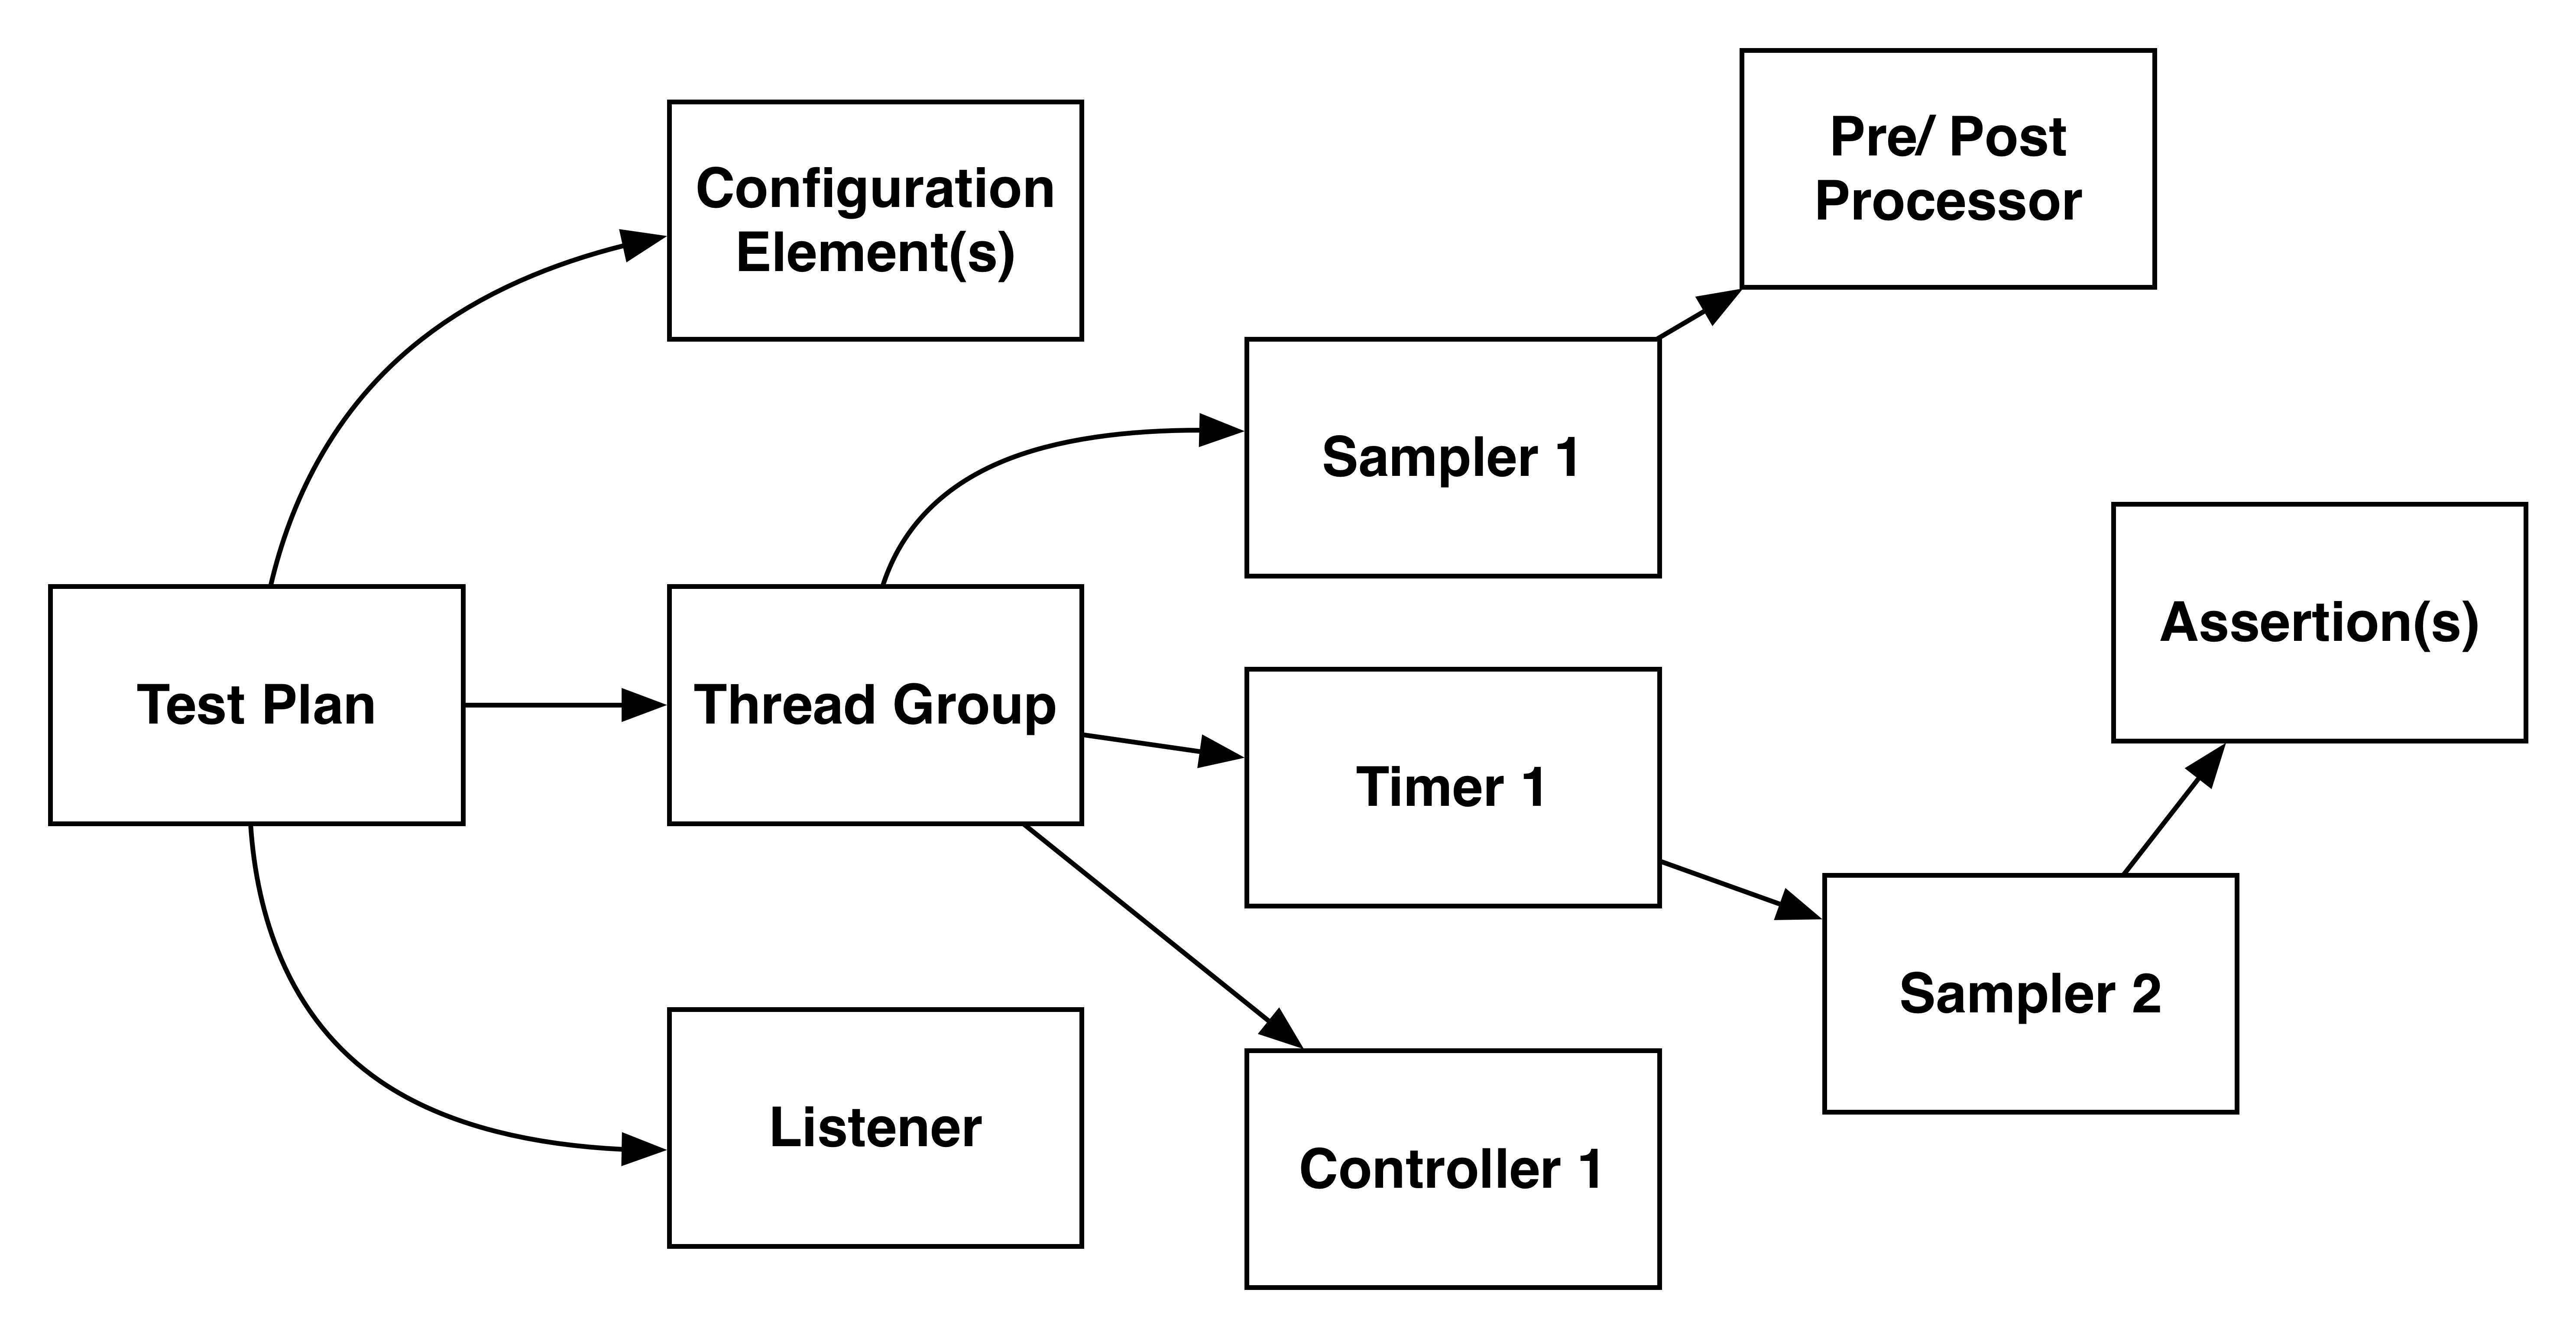
\includegraphics[width=0.5\textwidth]{./images/jmeteranatomy.png}
\caption{Anatomy of JMeter script \cite{Erinle2013}}
\label{fig:jmeteranatomy}
\end{figure}

Thread Groups represents the number of threads/users JMeter will use to execute the test plan. All controllers and samplers for a test must reside under a Thread Group. Other elements, such as listeners, may be placed directly under a test plan. Thread Group configurations provide options to specify the number of threads that will be used for the test plan, how long it will take for all threads to become active (ramp up), and the number of times to execute the test \cite{Erinle2013}.

Configuration elements work with a sampler, enabling requests to be modified or added to. Listeners are components  used to post process request data, storing the results of a test run making possible it to be further analyzed.  Listeners can be added anywhere in the test script, including directly under the test plan. They will collect data only from the elements at or below their level \cite{Erinle2013} \cite{Nevedrov2007} \cite{Halili2008}. 

Samplers allow JMeter to send requests to a server and wait for a response. Requests are processed in the order they appear in the tree. Timers allow JMeter   pause a certain amount of time before each sampler \cite{Nevedrov2007}  \cite{Halili2008}.

The main results presented by JMeter are:

\begin{itemize}
\item Response time : the elapsed time from just before sending the request to just after the last response has been received.
\item Latency: latency from just before sending the request to just after the first response has been received. Thus the time includes all the processing needed to assemble the request as well as assembling the first part of the response.
\item Connect Time: time it took to establish the connection, including SSL handshake. 
\item Median:  number which divides the samples into two equal halves. Half of the samples are smaller than the median, and half are larger. The Median is the same as the 50th Percentile.
\item 90\% Line (90th Percentile) is the value below which 90\% of the samples fall. The remaining samples too at least as long as the value. 
\item Standard Deviation:  measure of the variability of a data set. 
\end{itemize}
%\section{Combinatorial Optimization Algorithms in Load, Performance and Stress Tests}

The objective of combinatorial optimization algorithms consists of a set of  techniques for finding minimum or maximum values of a function of very many independent variables. This function, usually called the cost function or objective function, represents a quantitative measure e of the "goodness" of some complex system \cite{Kirkpatrick2007}. 

Afzal, Torkar and Feldt presents a systematic review of the use combinatorial  optimization algorithms in non-functional tests ( non-functional search-based testing). The review catalogs 30 studies of which 12 use combinatorial optimization algorithms to perform perform load, stress or performance tests. In Afzal et al. review, The most used algorithms are Genetic Algorithms and  Simulated Annealing \cite{Afzal2009a}.

This study aims to use genetic algorithms and simulated annealing algorithm in conjunction with the Tabu Search to perform performance, load and stress testing.

% quais algoritmos vao ser discutidos?
% porque estes?

\subsection{Genetic Algorithms}

Genetic algorithms (GA) is an adaptive search techniques based on the processes of natural genetics and Darwin’s theory of biological evolution. GA are characterized by  work in parallel on a number of potential solutions, the population of individuals. In every individual, permissible solution values for the variables of the optimization problem are coded. The concept of genetic algorithms is related with  successive generations of increasingly better combinations which significantly increase the overall performance of a system \cite{Sullivan} \cite{goldberg1989messy}.

\subsection{Simulated Annealing Algorithm}

Simulated Annealing  algorithm was motivated by the cooling of molten metal. After slow cooling (annealing), the metal arrives at a low energy state.
Inherent random fluctuations in energy allows the annealing system to escape local energy minima to achieve the global minimum. But if cooled very quickly, it might not escape local energy minima and when fully cooled it may contain more energy than annealed metal. Simulated annealing attempts to minimize some analogue of energy in a manner similar to annealing to find the global minimum \cite{Goffe1994}.

\subsection{Tabu Search Algorithm}

Tabu search is a strategy for solving combinatorial
optimization problems. It is an adaptive procedure with the ability to make use of many other methods, such as linear programming algorithms and specialized heuristics \cite{Glover1989}. The Fig. \ref{fig:tabualg} presents the basic workflow of Tabu Search algorithm. The first step is to create a initial solution and a set of neighbours. The solutions are evaluated and the best feasible solution is chosen.

\begin{figure}
\centering
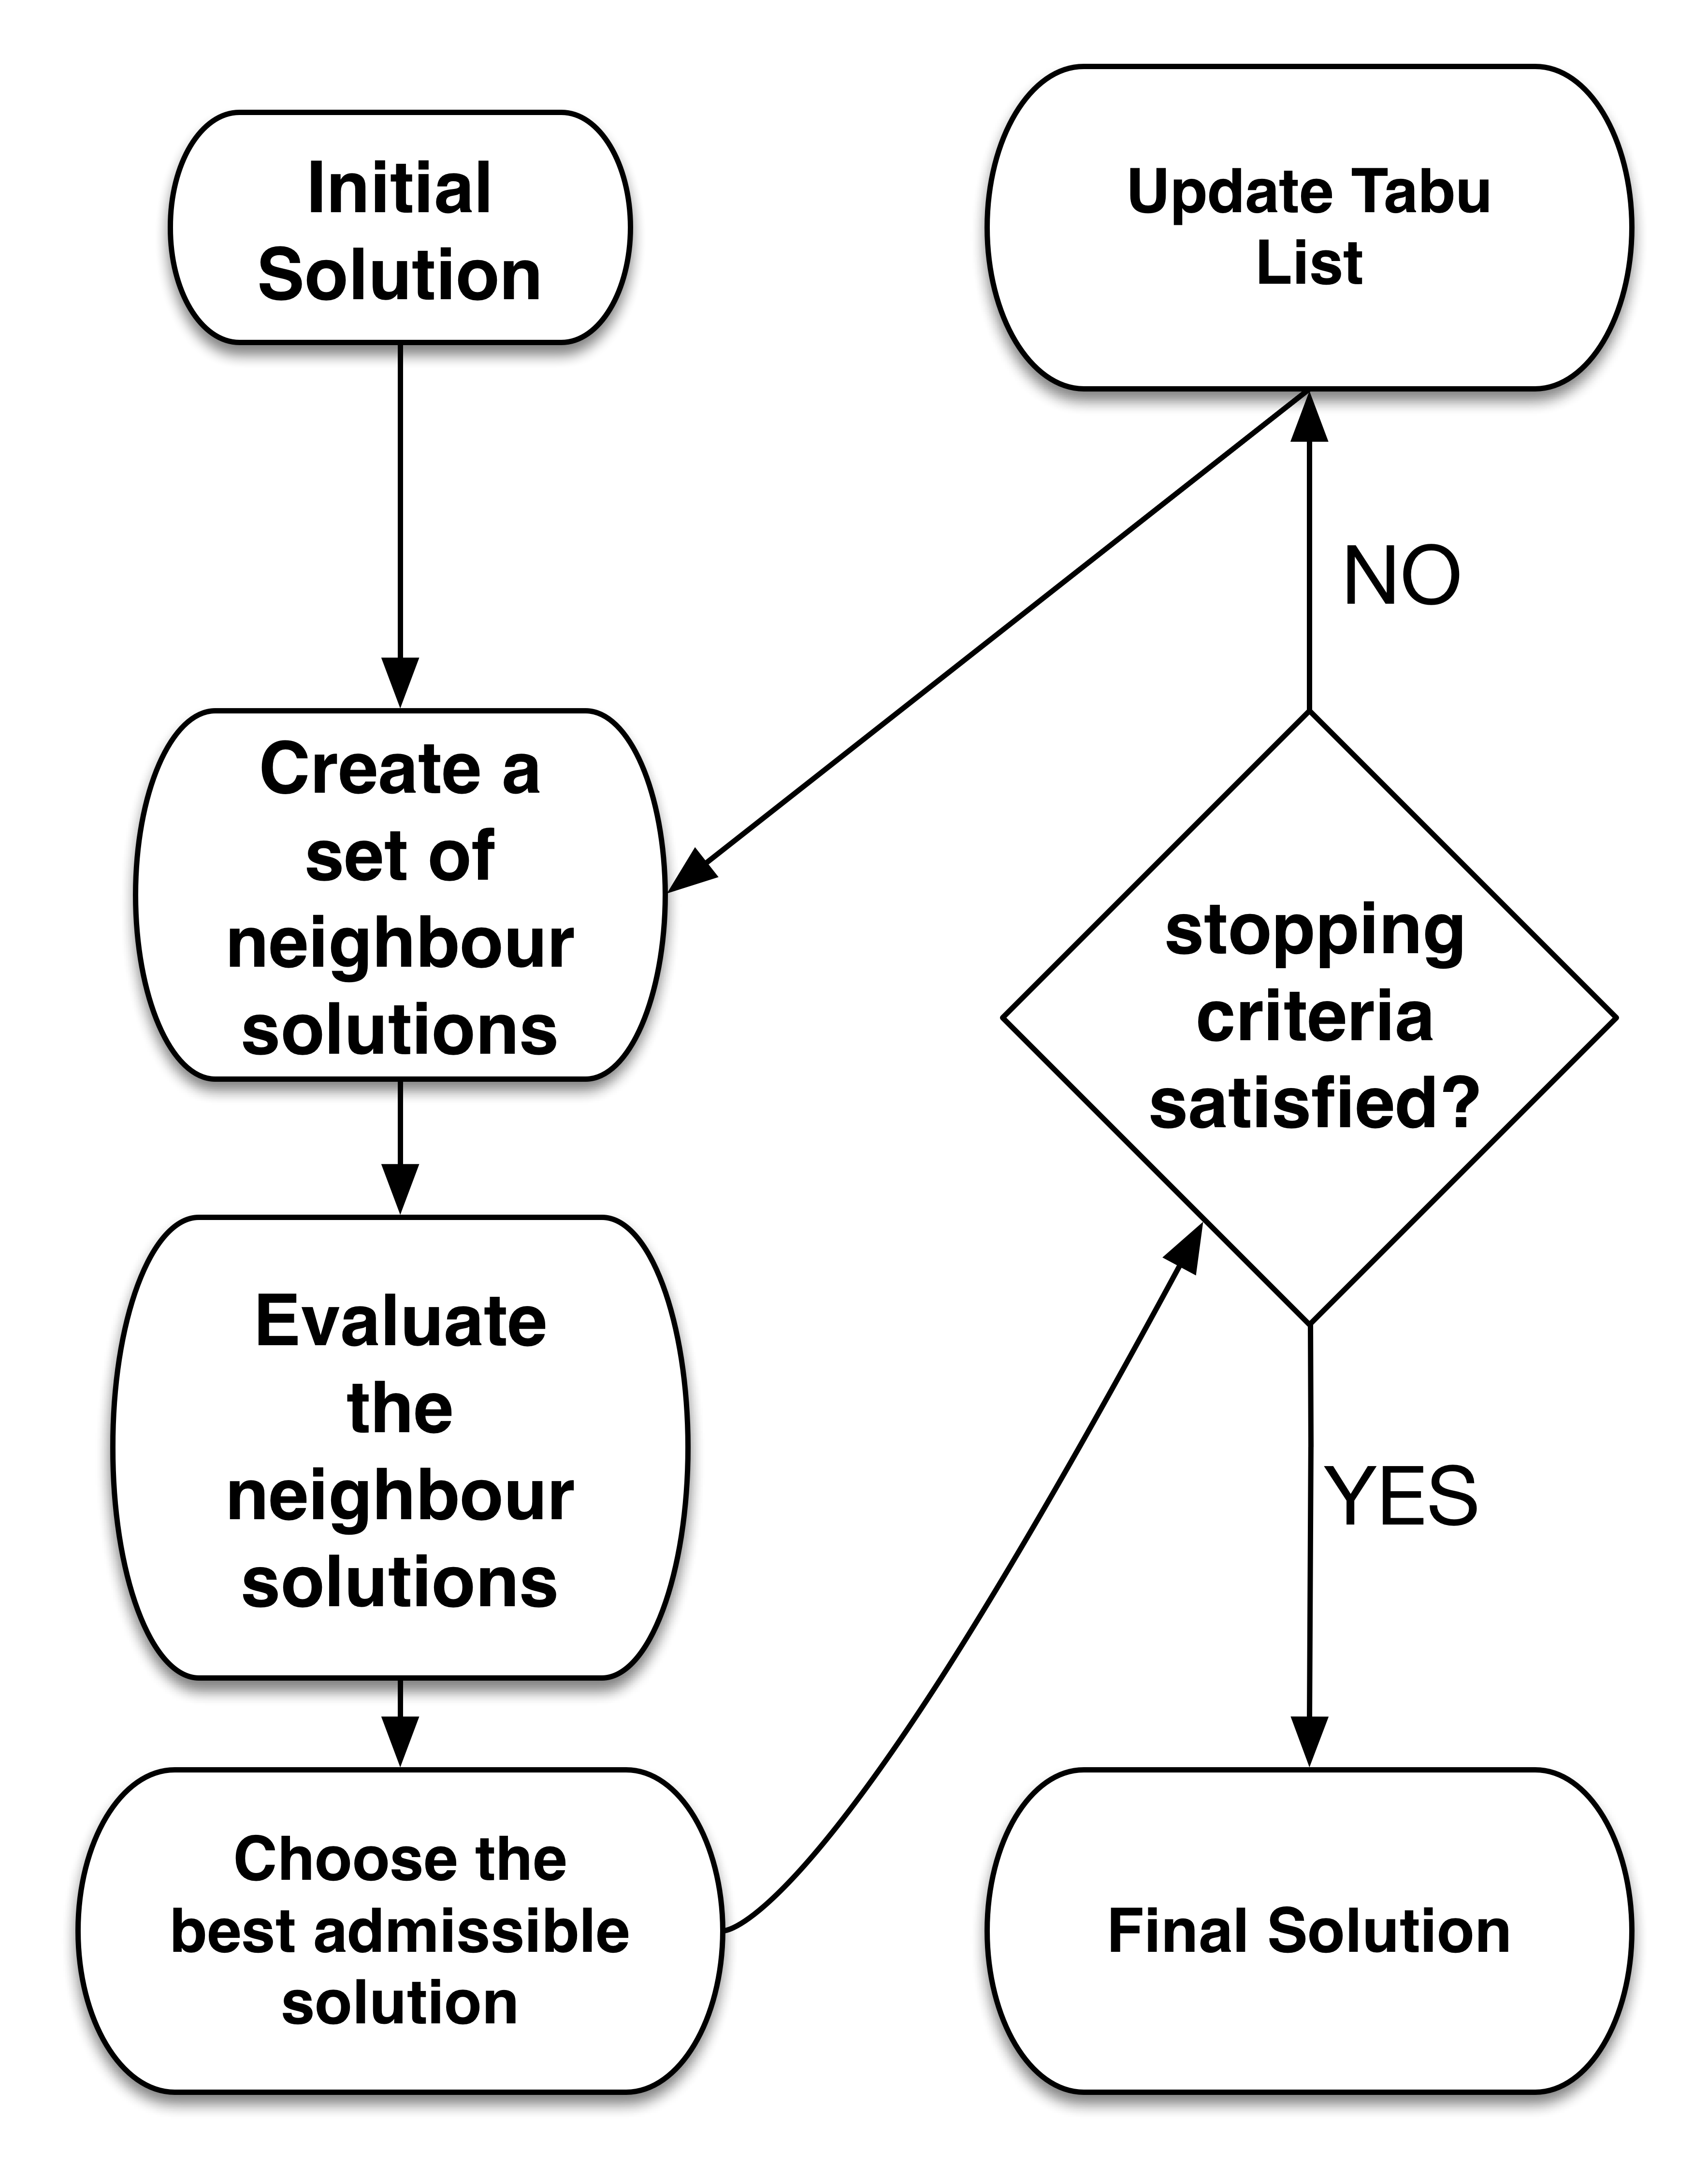
\includegraphics[width=0.4\textwidth]{./images/tabualgorithm.png}
\caption{Tabu Search Algorithm}
\label{fig:tabualg}
\end{figure}


Tabu search  classify a subset of the moves in a neighborhood as forbidden. A tabu list records forbidden moves, which are referred to as tabu moves. A neighborhood is constructed to identify adjacent solutions that can be reached from current solution \cite{reeves1993modern}. 

Tabu restrictions are subject to an important exception.  When a tabu move has a evaluation where it would result in a solution better than any visited so far, then its tabu classification may be overridden.  A condition that allows such an override to occur is called an aspiration criterion \cite{reeves1993modern}. 

The Tabu search uses three main strategies \cite{reeves1993modern}:

\begin{itemize}
\item Forbidding strategy: control what enters the tabu list;
\item Freeing strategy: control what exits the tabu list and when; and
\item Short-term strategy: manage interplay between the forbidding strategy and freeing strategy to select trial solutions.
\end{itemize}
\section{Hybrid Metaheuristc}


A large  number of researchers have recognized the advantages and huge potential Building
hybrid mathematical programming methods and metaheuristics.
The main motivation to create hybrid Metaheuristics is to exploit the complementary character of different optimization strategies. In fact, choosing an adequate combination of algorithmic can be the key for achieving top performance in solving many hard optimization problems \cite{Puchinger2005} \cite{Blum2012}.


There are two main categories of metaheuristc combinations: Collaborative Combinations and Integrative Combinations. The Fig. \ref{fig:metaheuristc} presents the two main categories of Hybrid MetaHeuristc \cite{Puchinger2005}.

\begin{figure}[h]
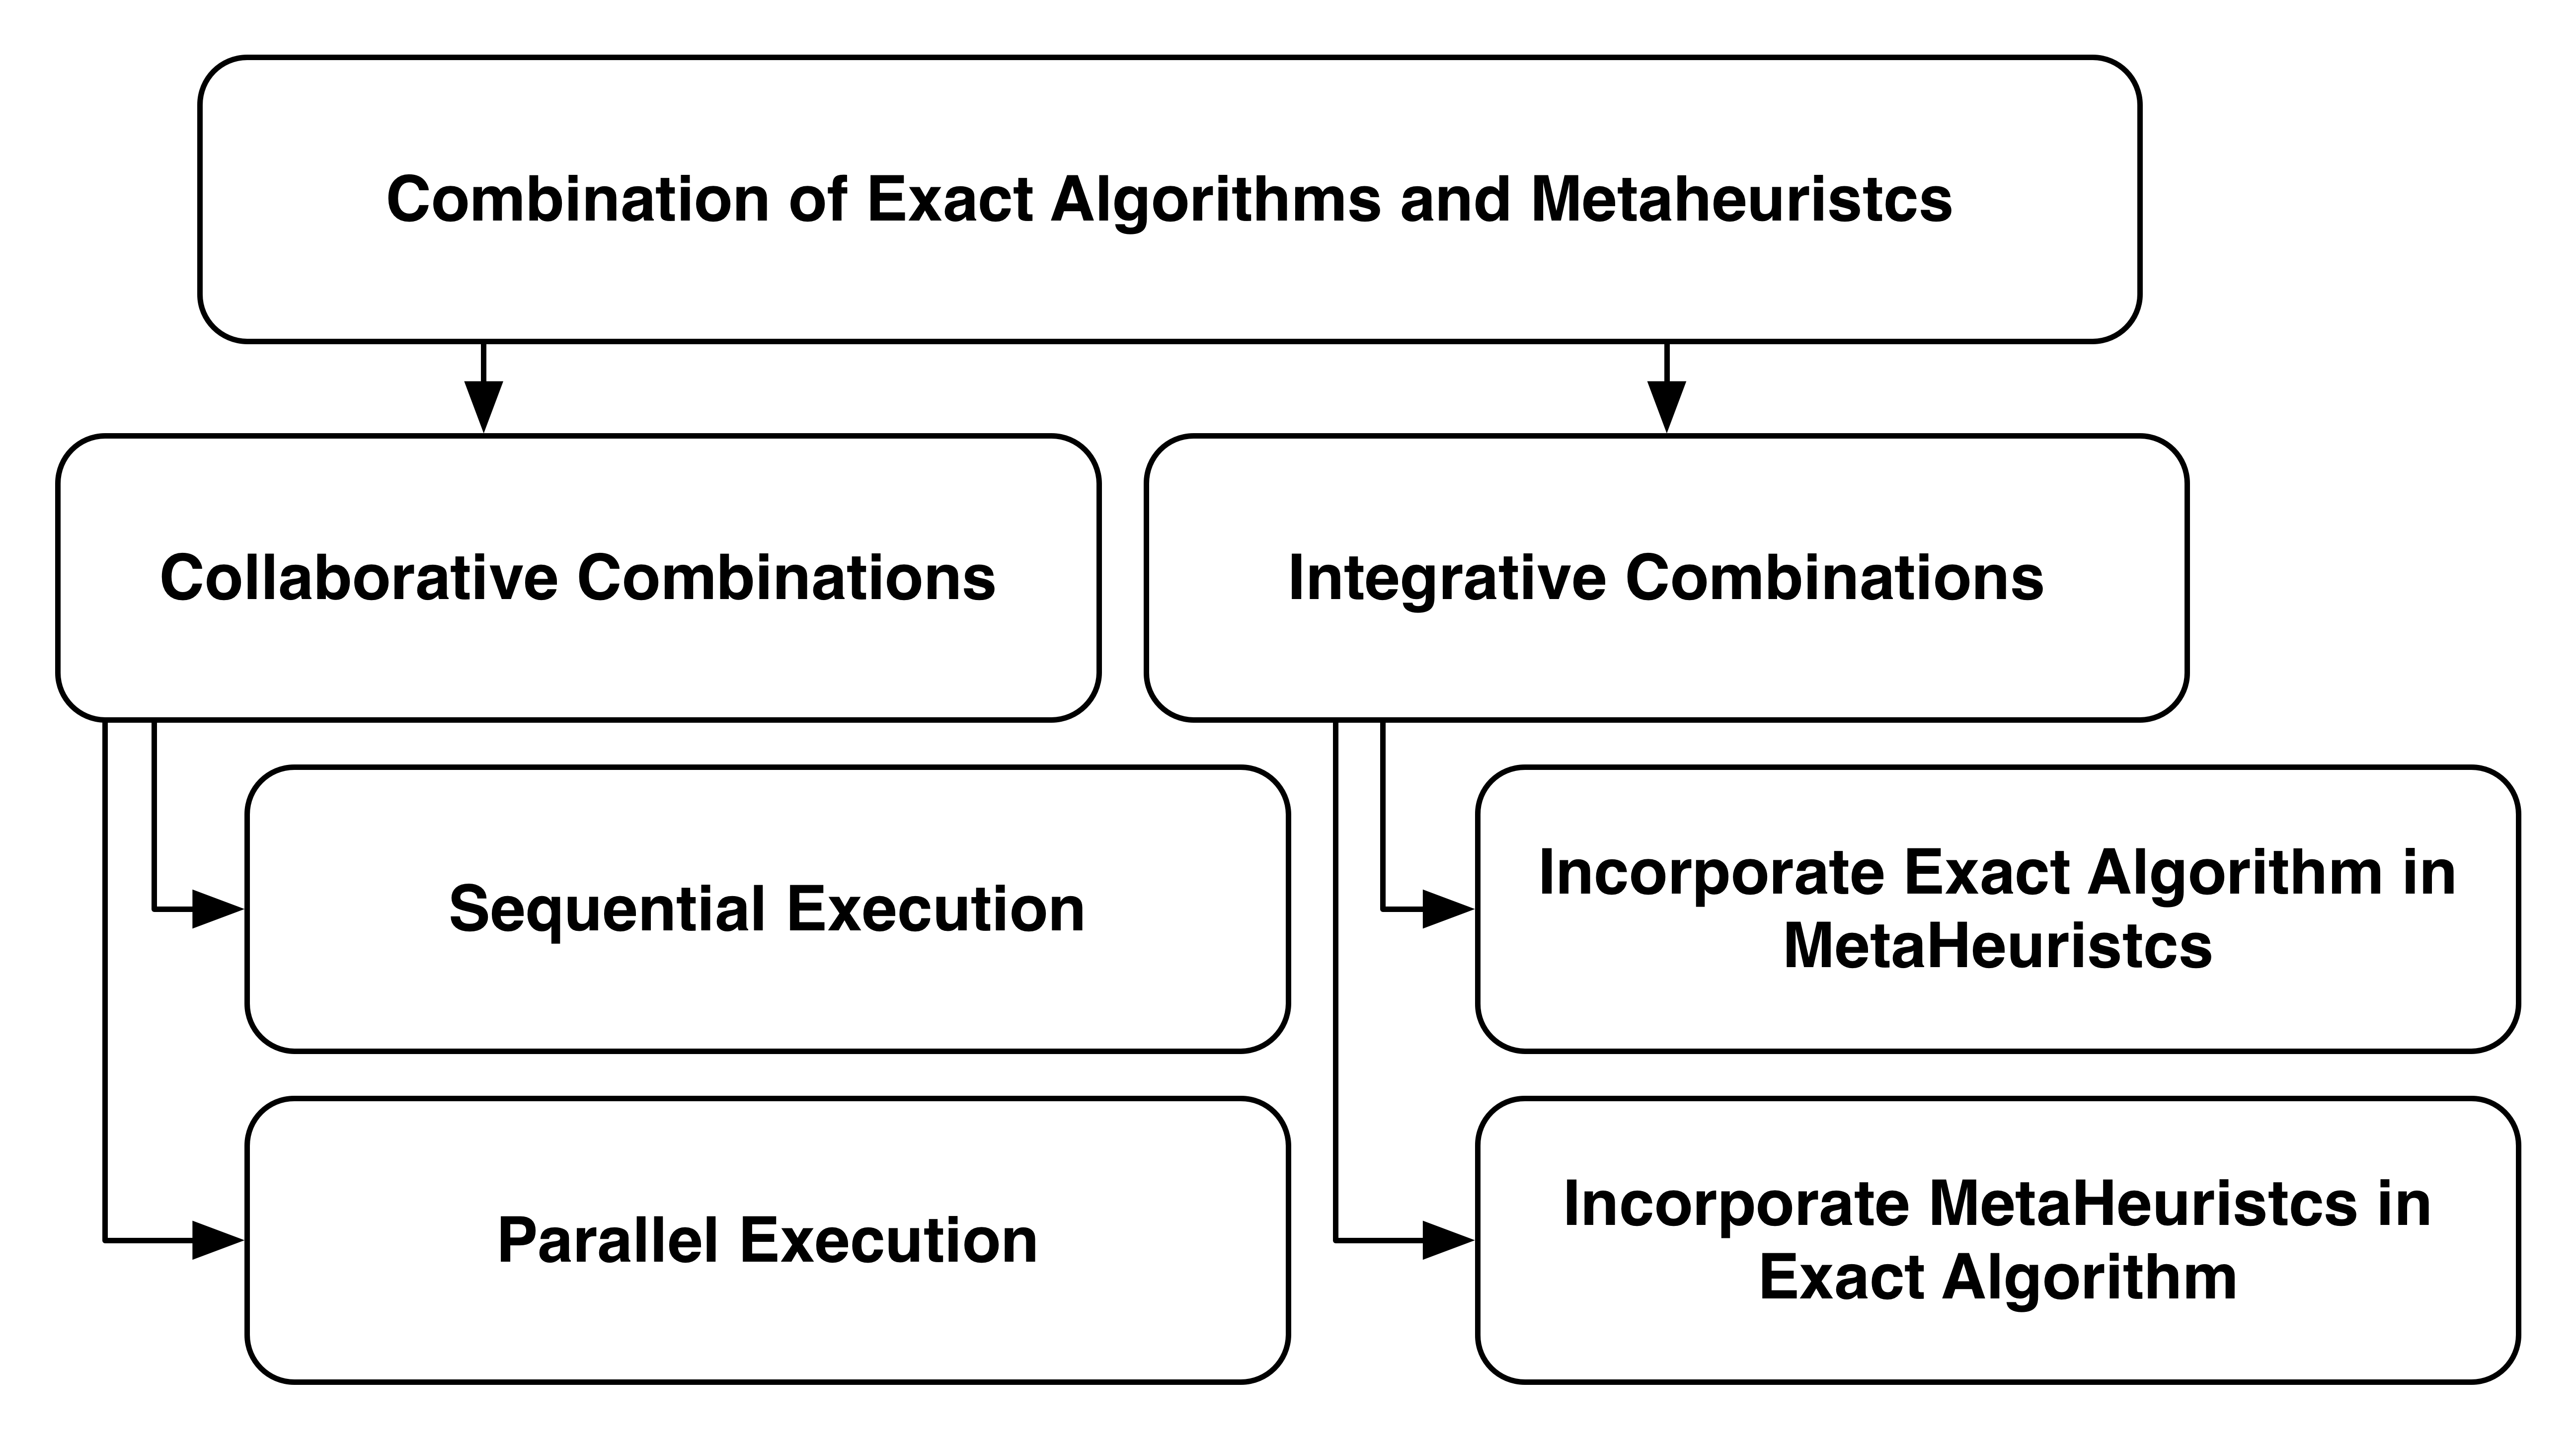
\includegraphics[width=0.5\textwidth]{./images/metaheuristcs.png}
\caption{Categories of metaheuristc combinations \cite{Puchinger2005} }
\label{fig:metaheuristc}
\end{figure}

Collaborative Combinations uses a approach where the  algorithms exchange information, but are not part of each other. In this approach,  algorithms may be executed sequentially or in parallel. The presented research work uses a type of  Collaborative Combination with Sequential Execution.


\section{Evolutionary Test in Load, Performance and Stress Tests}

The search for the longest execution time is regarded as a discontinuous, nonlinear, optimization problem, with the input domain of the system under test as search space \cite{Sullivan}. The main objective of evolutionary testing in performance,stress and load tests is to find test scenarios which produce execution times violating the timing constraints specified. If a temporal error is found, the test was successful \cite{Sullivan}. The application of evolutionary algorithms to load, performance and stress tests involves finding the best and worst case execution times (BCET, WCET) to determine if timing constraints are fulfilled \cite{Afzal2009a}. 

Evolutionary tests uses a cost (fitnesse) function to select the best individuals. There has two measurement units normally associated with the fitnesse function in load, performance or stress test: Processor Cycles and Execution Time. The Processor Cycles approach describes a fitness function in terms of processor cycles. The Execution Time approach involves executing the application under test measuring the execution time \cite{Afzal2009} \cite{tracey2000search}.
% * <naubergois@gmail.com> 2015-09-17T01:17:52.488Z:
%
%  Rever esse paragrafo
%
The Figure \ref{fig:comparison}  shows a comparison between the presented research work and the load, performance and stress test researches presented by Afzal et. al. \cite{Afzal2009}. Afzal's work was added with some of the latest research in the area (\cite{Garousi2006} \cite{Garousi2010}). The x axis represents the type of tool used ( Prototype or Functional Tool )  and the y axis presents the metaheuristic used by each research (Genetic Algorithm, Tabu Search, Simulated Annnealing or a Customized Algorithm). The Figure also divides the researches by the type of function fitnesse (Execution Time or Processor Cycles). Most research is limited to making prototypes on genetic algorithms. The presented research work is distinguished from others by having a functional tool using a hybrid approach. 

% * <naubergois@gmail.com> 2015-09-17T01:22:09.554Z:
%
%  Customized Algorithm
%

\begin{figure}[h]
\centering
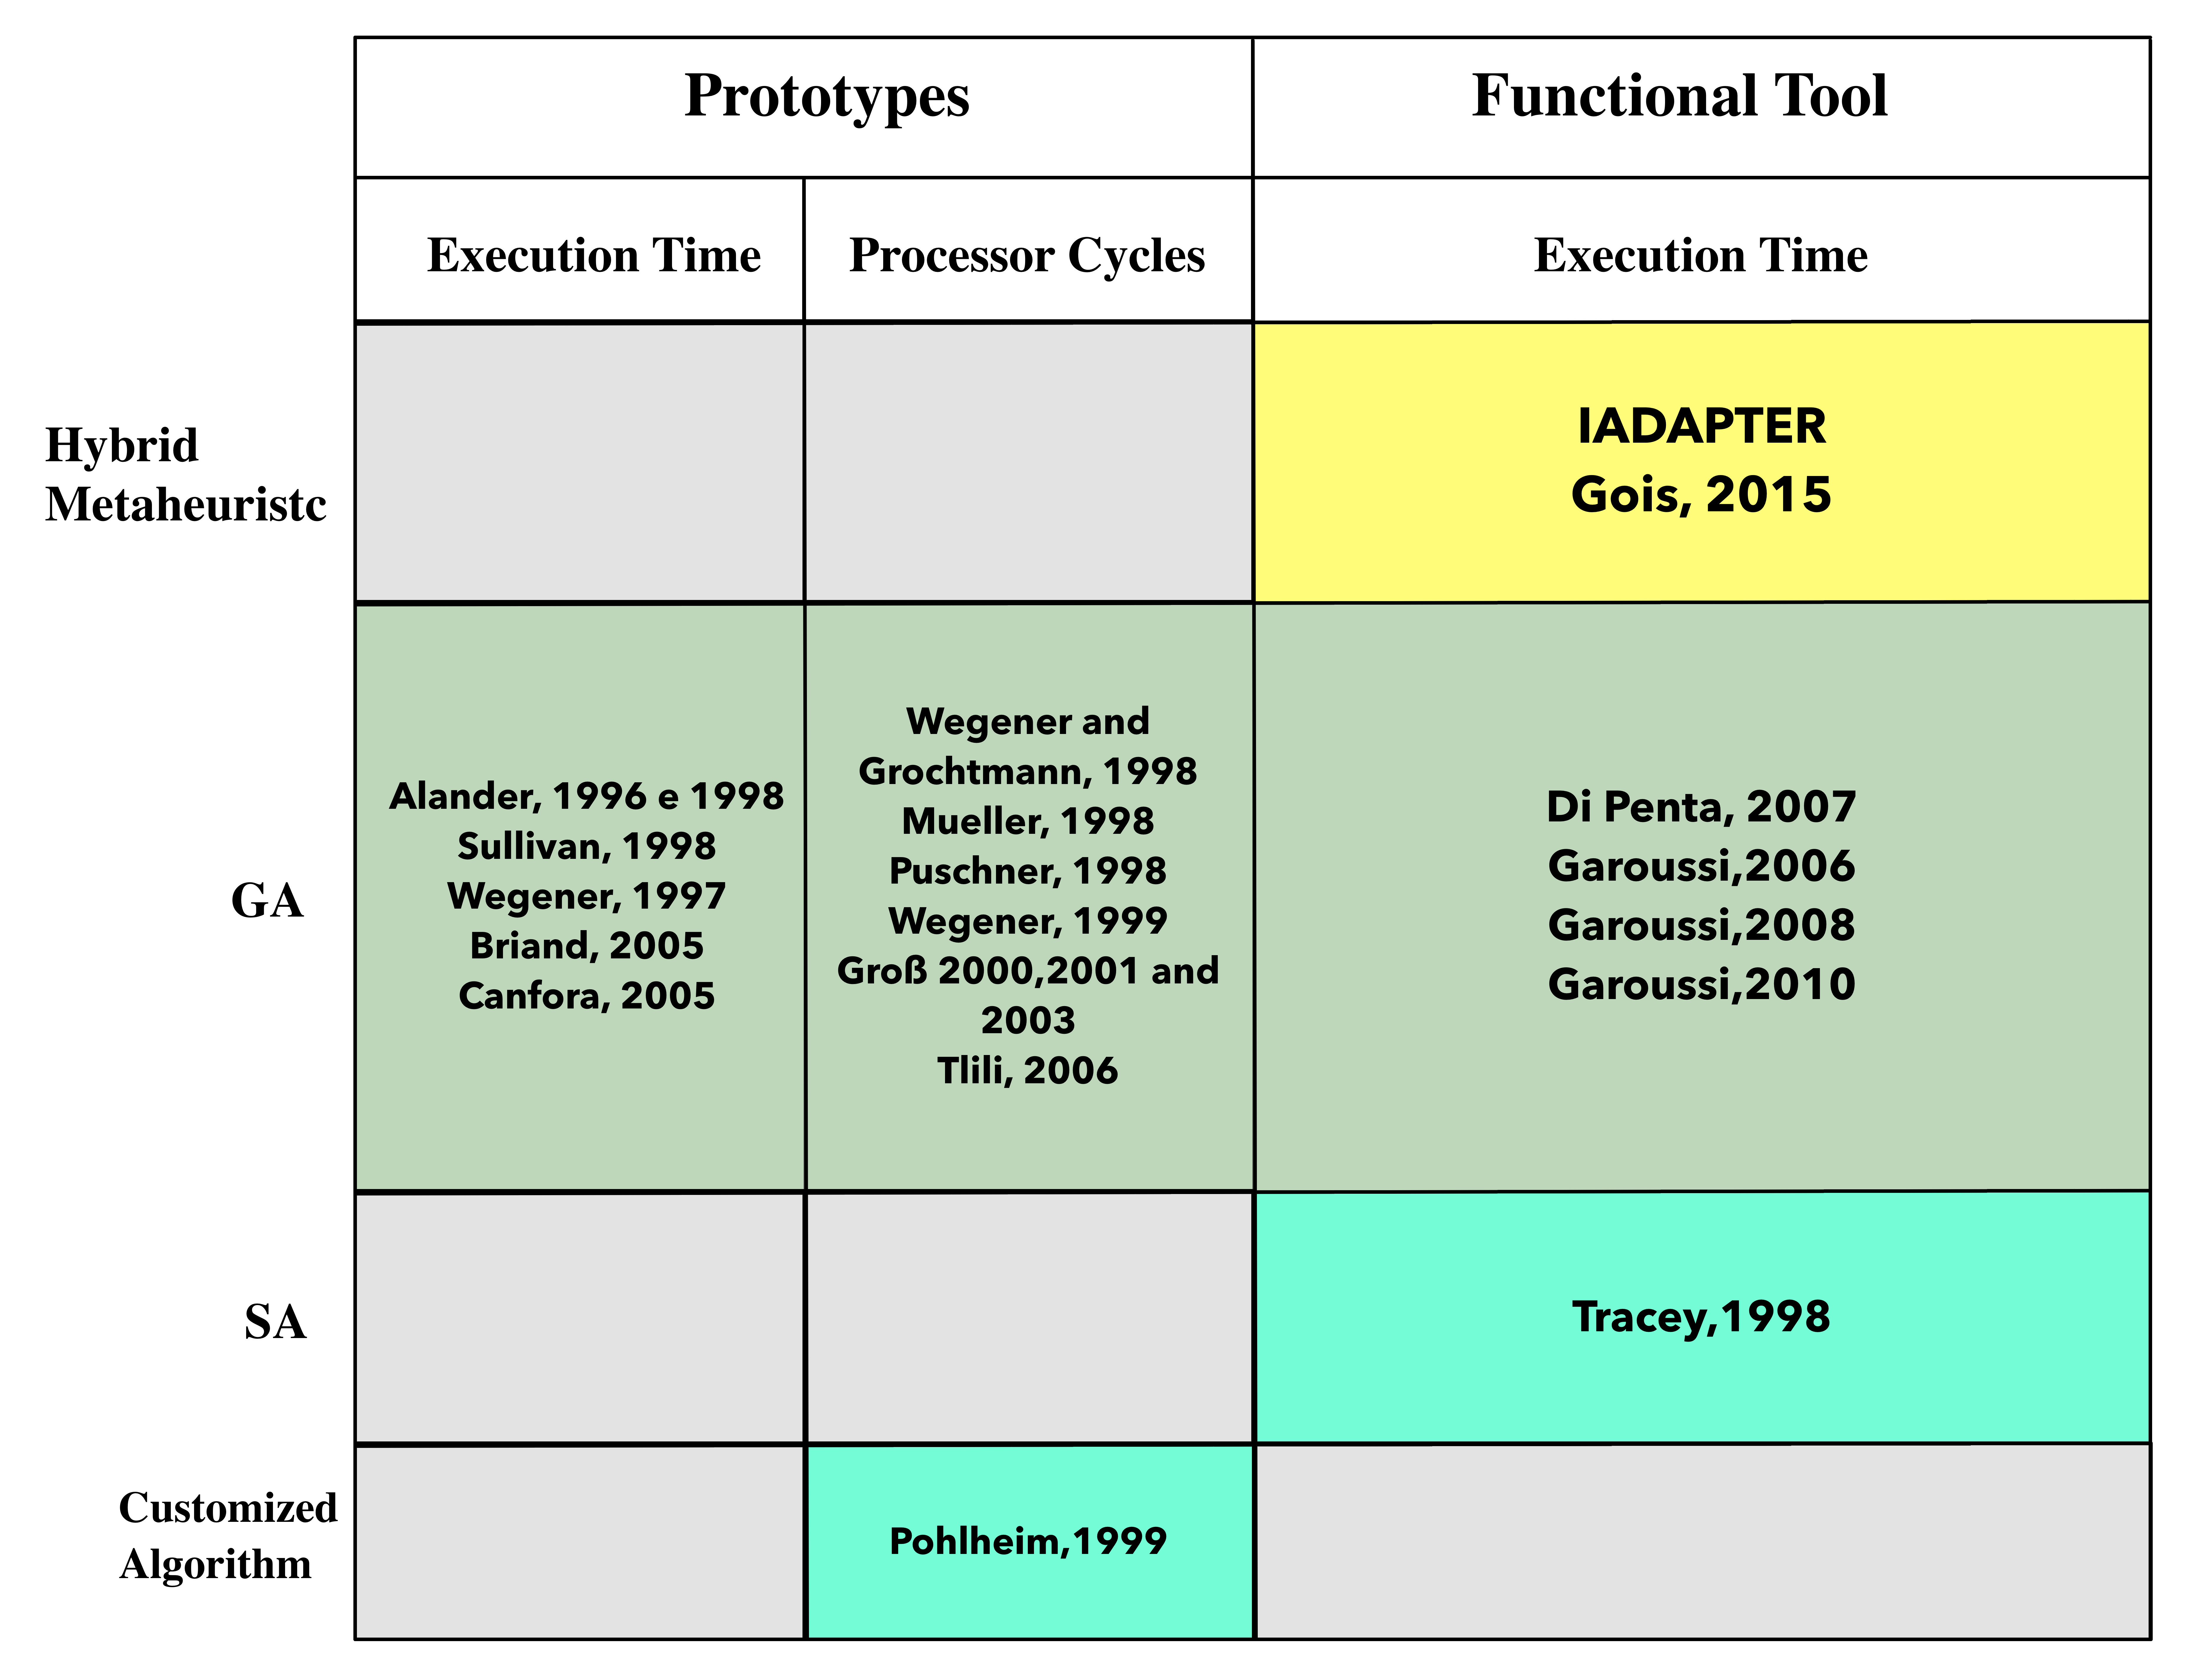
\includegraphics[width=0.5\textwidth]{./images/comparativo1.png}
\caption{
Distribution of the researches over range of applied metaheuristics}
\label{fig:comparison}
\end{figure}
\section{IAdapter}

IAdapter is a JMeter Plugin to perform evolutionary load, performance or stress tests. JMeter is a desktop application, designed to test and measure the performance and functional behavior of applications \cite{Nevedrov2007}.

The IAdapter plugin makes it possible to create a generative model that evolves during the test. The IAdapter model uses Genetic Algorithm, Tabu Search and Simulated Annealing in two different approaches.  The first approach uses the three algorithms independently and the second approach uses the three algorithms collaboratively (Hybrid Metaheuristic approach).

In the first approach , the algorithms do not share their best individuals among themselves. Each algorithm evolves in a separate way (Fig. \ref{fig:firstaproach}). The second approach use the algorithms in a collaborative mode (Hybrid Metaheuristic). In this approach, the three algorithms share their best individuals found (Fig. \ref{fig:secondapproach}).

The next subsections present details about the used metaheuristcs algorithms (genotype representation and fitnesse function) and the IAdapter components.

\begin{figure}[h]
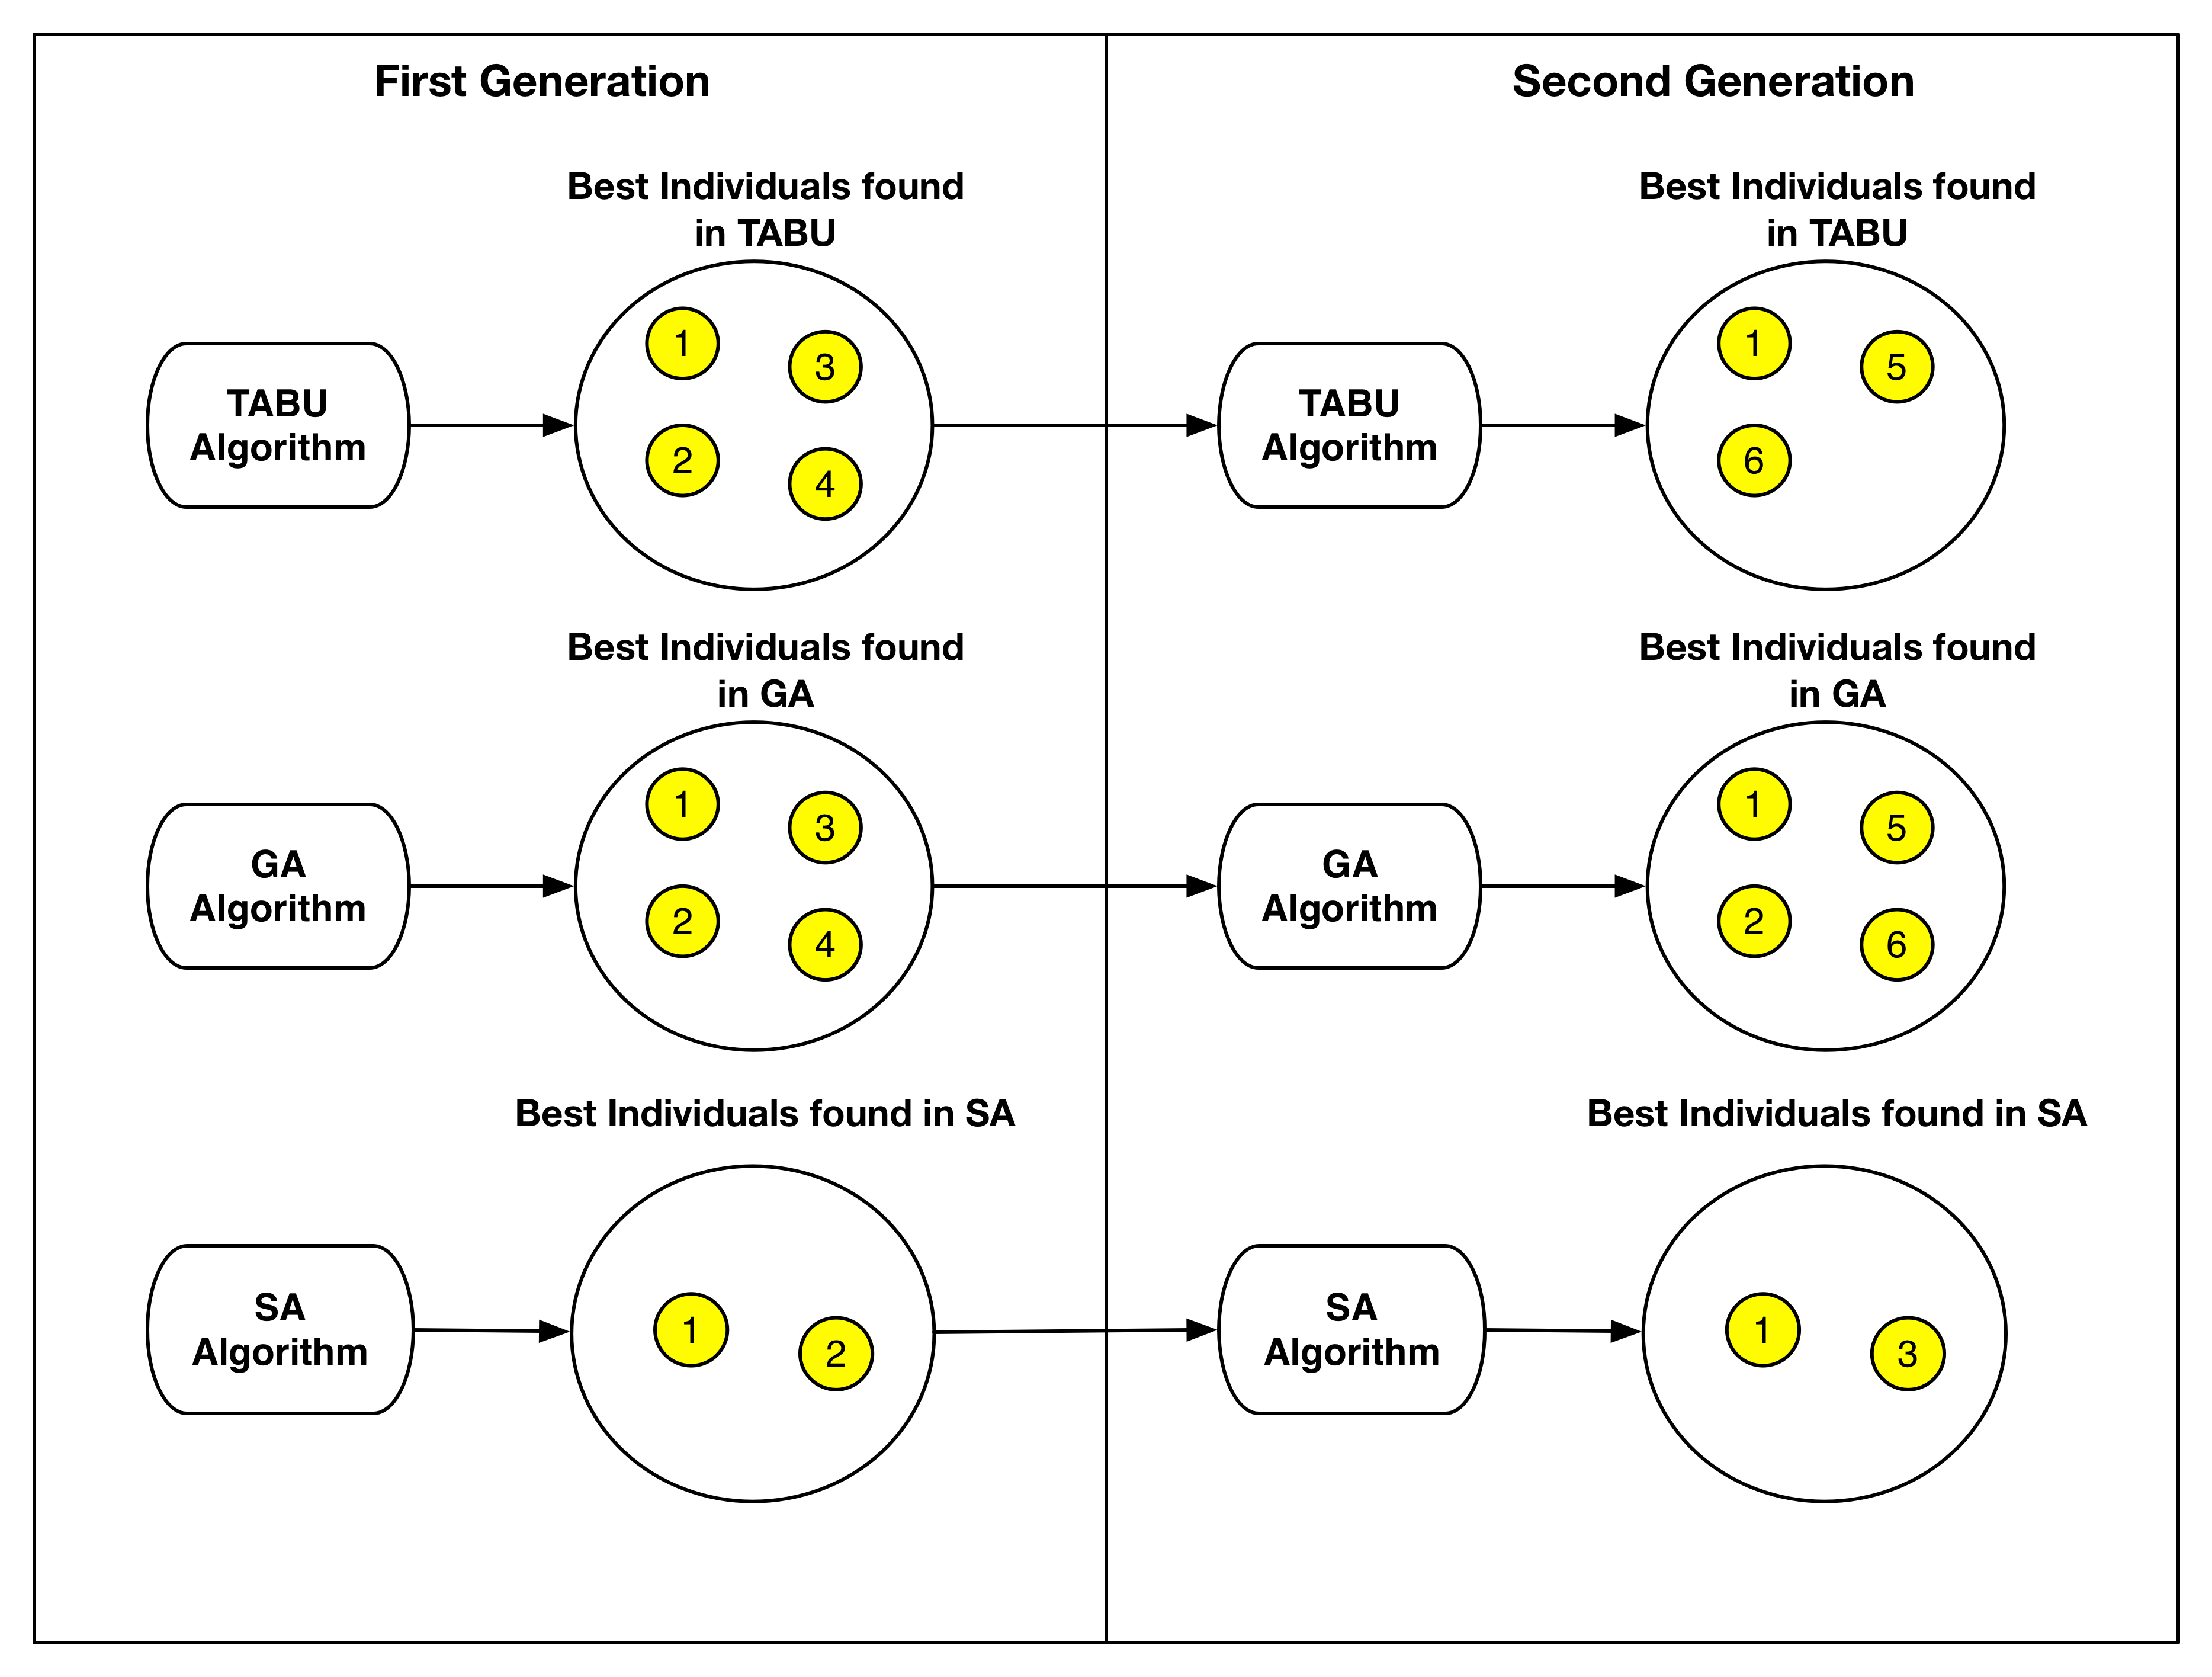
\includegraphics[width=0.5\textwidth]{./images/independ.png}
\caption{Use of the algorithms independently}
\label{fig:firstaproach}
\end{figure}
\begin{figure}
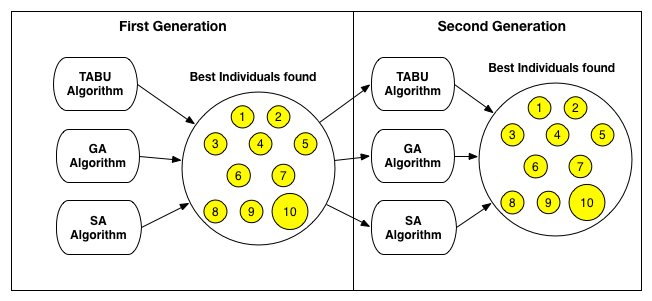
\includegraphics[width=0.5\textwidth]{./images/collaborative.png}
\caption{Use of the  algorithms collaboratively}
\label{fig:secondapproach}
\end{figure}

\subsection{Genotype representation}

The Genotype representation is composed by a linear vector with 23 genes. The first gene represents the name of individual. The second gene presents the  algorithm (Genetic Algorithm, Simulated Annealing or Tabu Search) used by the individual. The third gene represents the type of test (Load, Stress or Performance). Next genes represent 10 scenarios and their numbers of users. Each scenario is an atomic operation, the scenario must log in the application, run the task goal and undo any changes performed, returning the application to it's original state. 

The Fig. \ref{fig:genomarepresentation} presents the genome representation and  a example using the crossover operation. In the example, the genotype 1 has the Login scenario with 2 users; the Form scenario with 0 users and the Search scenario with 3 users. The genotype 2 has the Delete scenario with 10 users; the Search scenario with 0 users and the Include scenario with 5 users. After the crossover operation, We obtain a genotype with  Login scenario with 2 users; the Search scenario with 0 users and the Include scenario with 5 users.

\begin{figure}[h]
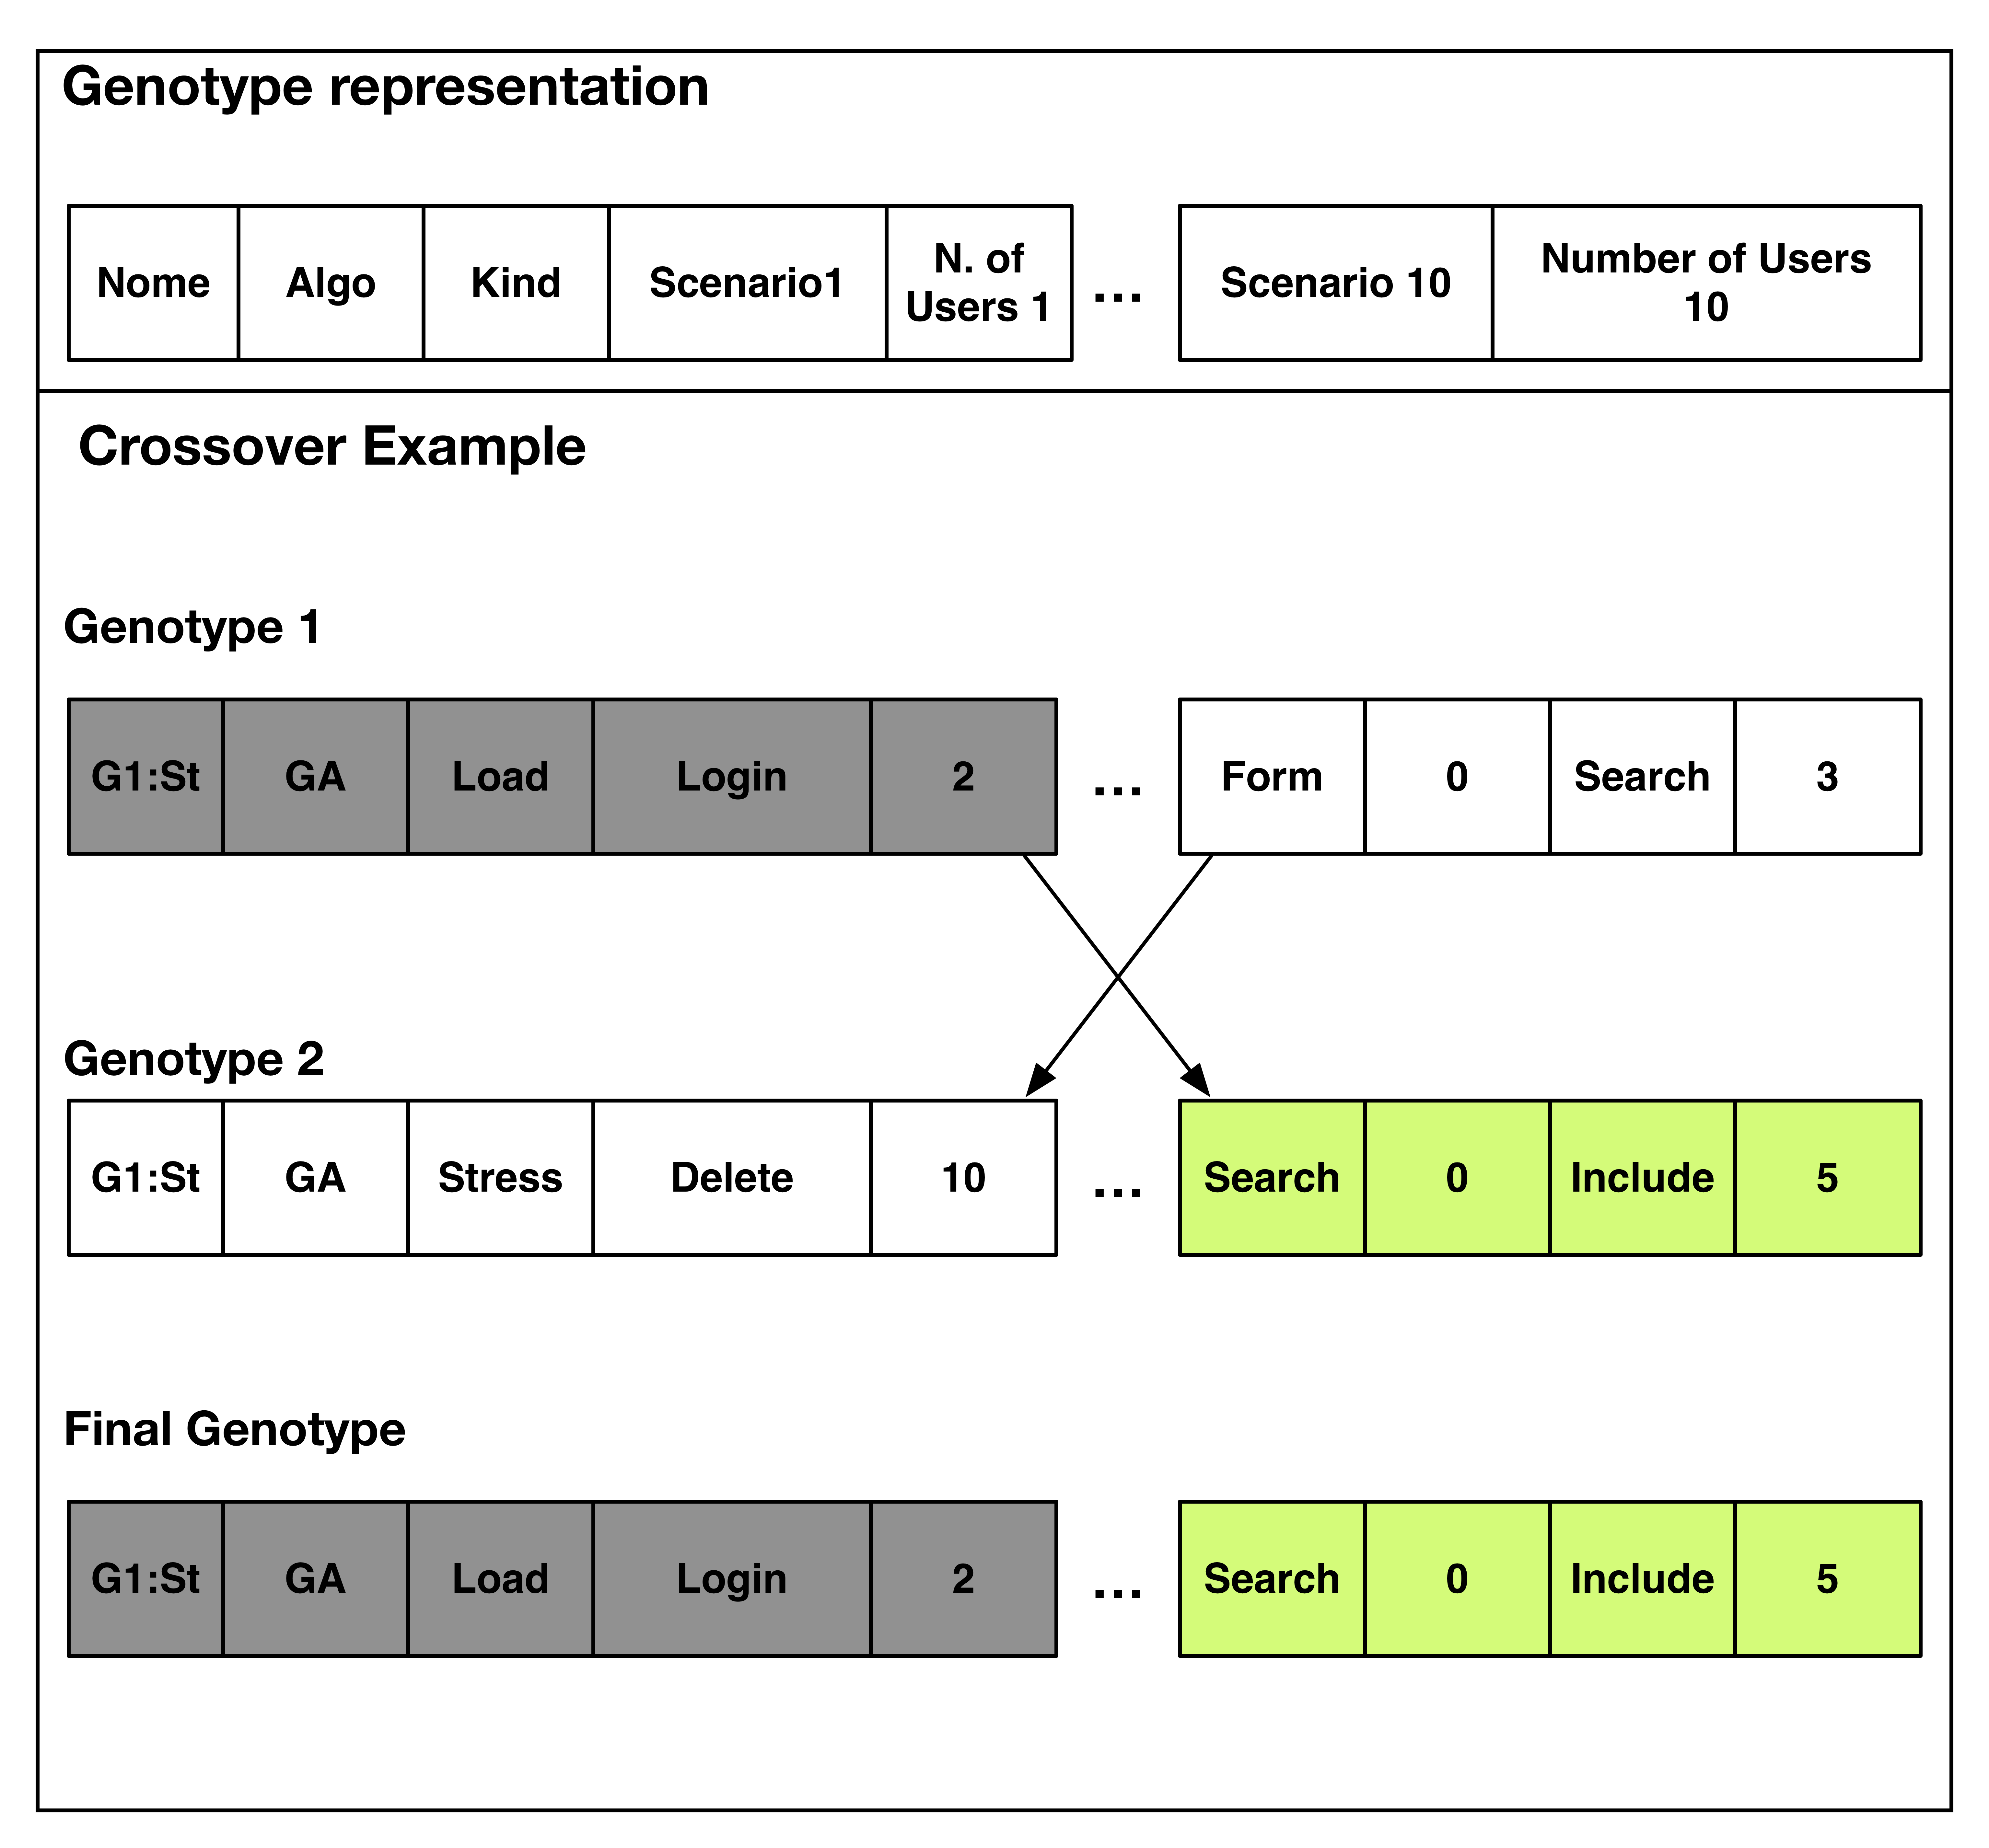
\includegraphics[width=0.5\textwidth]{./images/genomerepresentation.png}
\caption{Genotype representation and crossover example}
\label{fig:genomarepresentation}
\end{figure}

The Fig. \ref{fig:neighbourtaby} shows the strategy used by the IAdapter to obtain the genotype of the neighbours for the Tabu Search and Simulated Annealing algorithms.  The neighbours are obtained by the modification of a single cromossome (scenario or  number of users) in the genotype.

\begin{figure}[h]
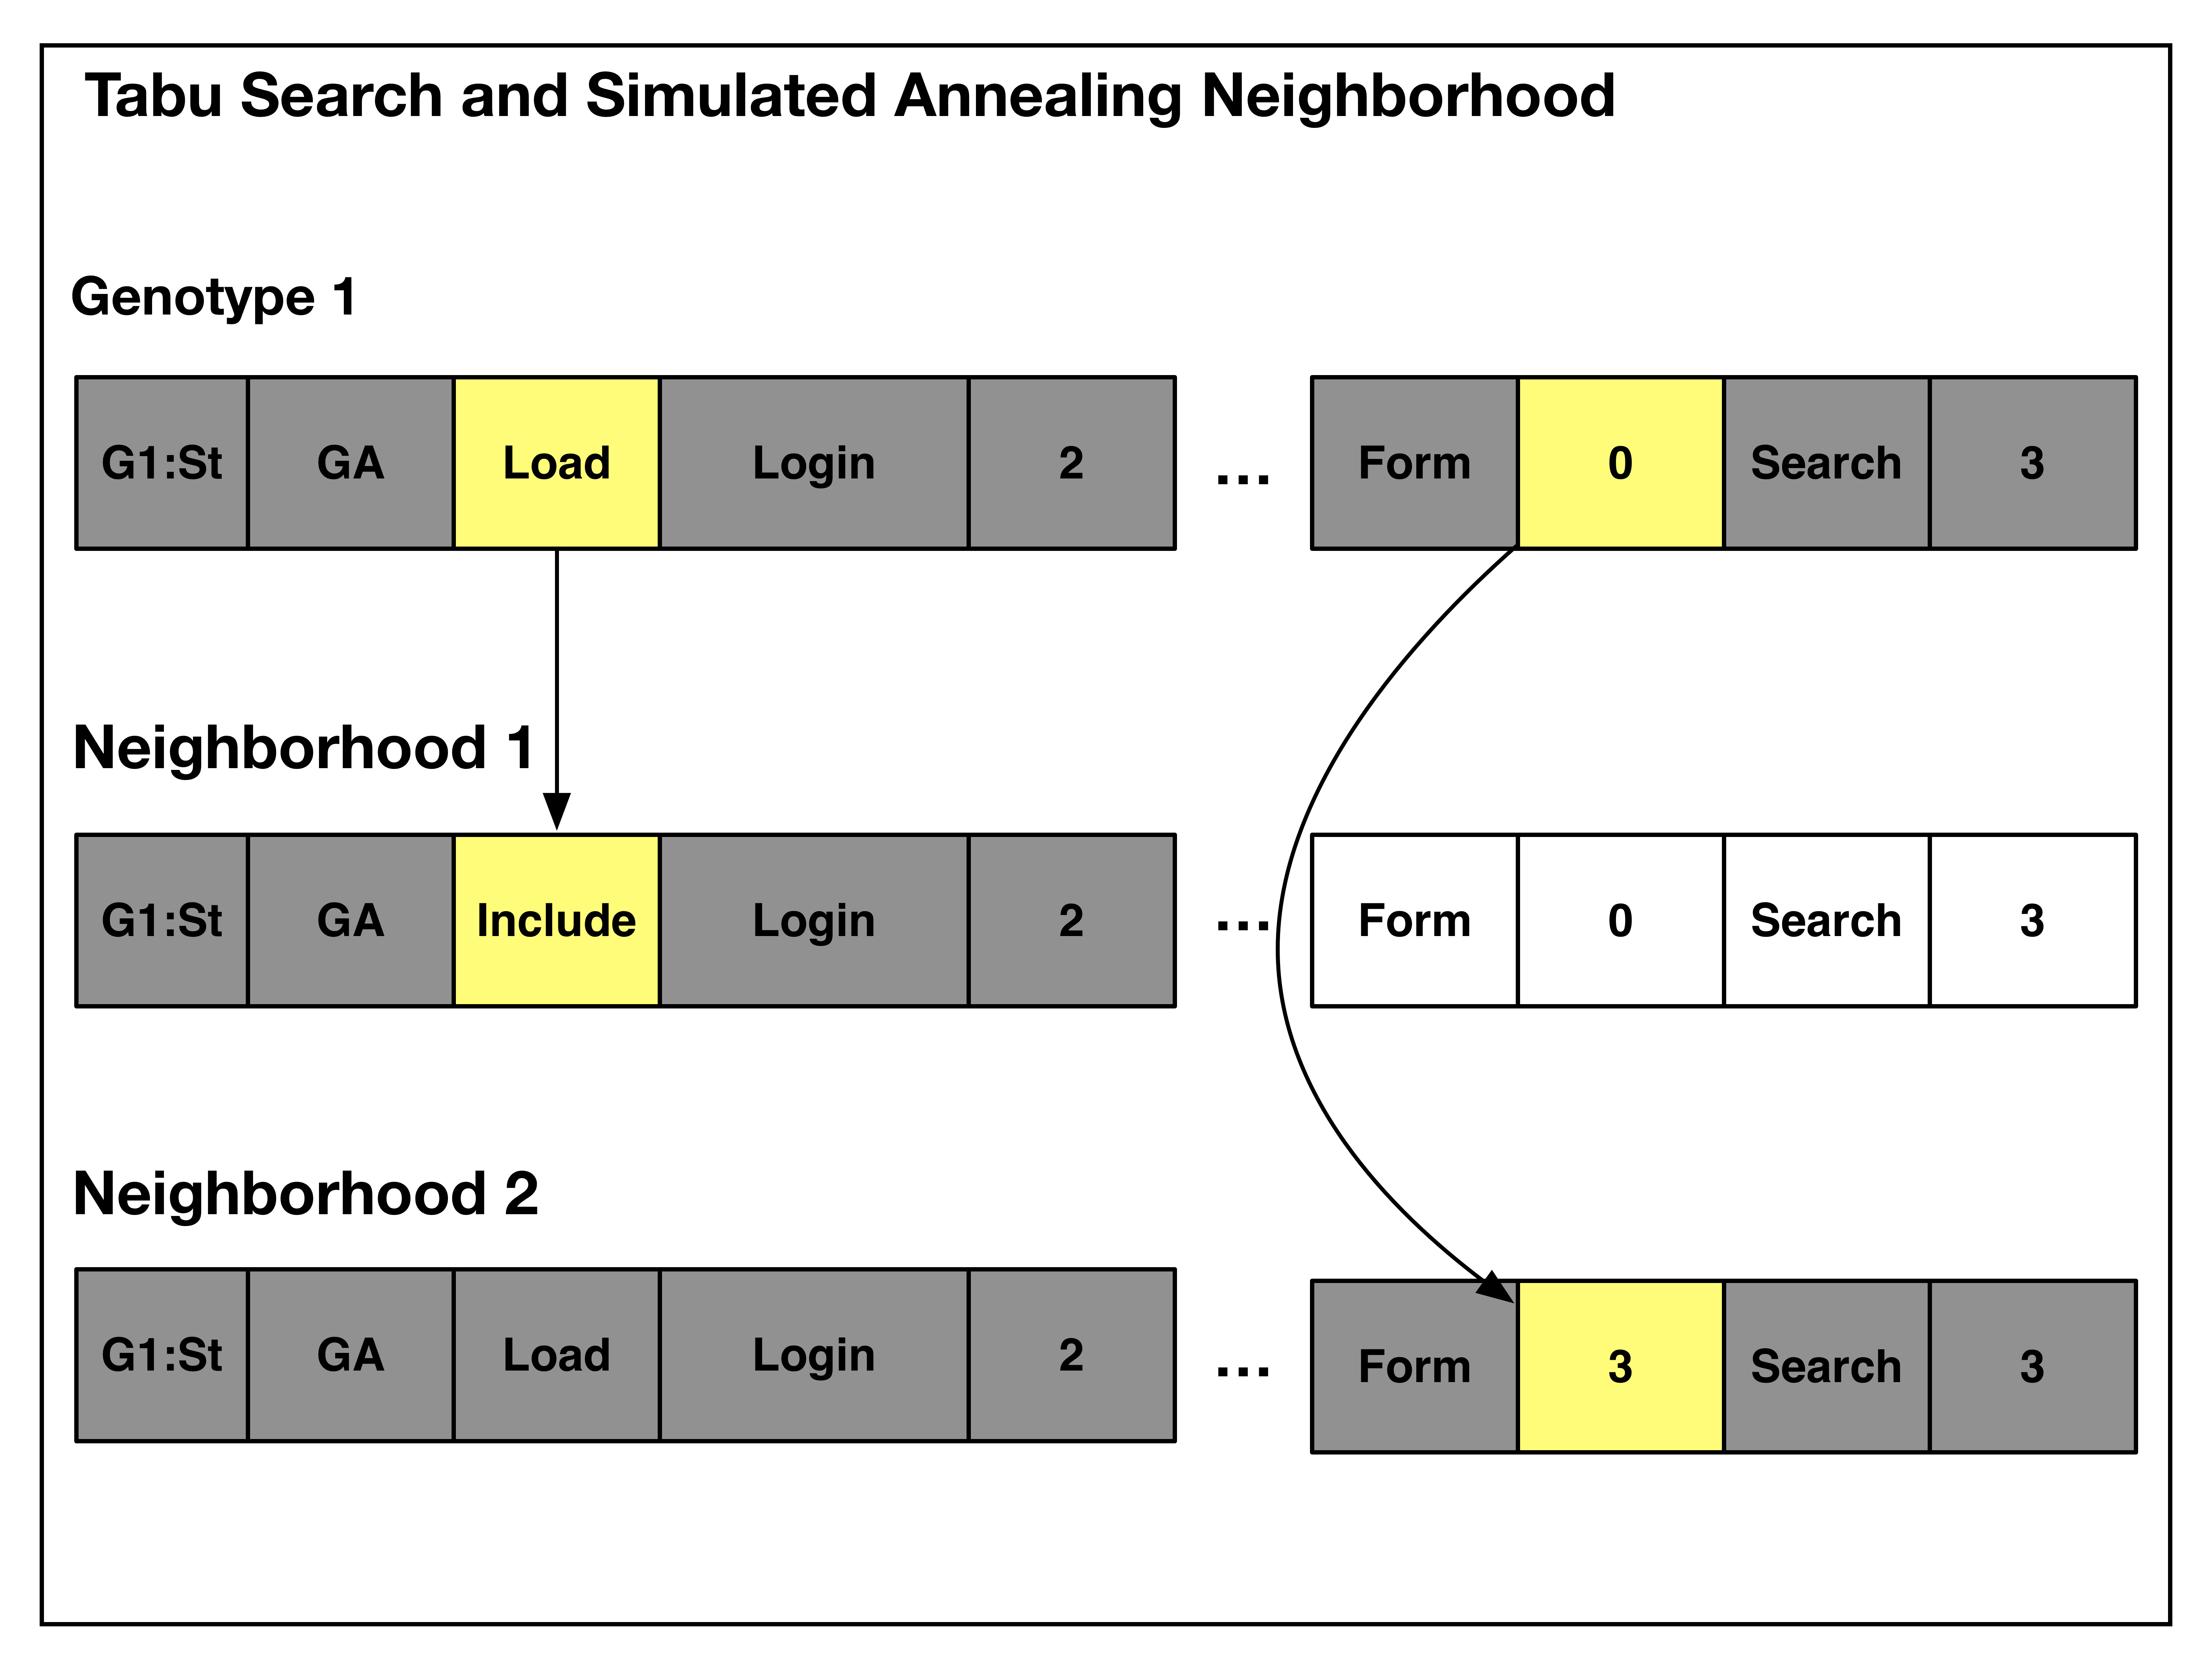
\includegraphics[width=0.5\textwidth]{./images/TabuNE.png}
\caption{Tabu Search and Simulated Annealing neighbour strategy}
\label{fig:neighbourtaby}
\end{figure}


\subsection{Objective (Fitnesse) Function}

The IAdapter is a tool to be used with the independent testing teams in various situations where the team has no direct access to the environment where the application under test was installed. Therefore,  The IAdapter uses a measurement approach to the definition of the fitnesse function. The fitnesse function applied to IAdapter solution is governed by the following equation:

\begin{equation}
\begin{aligned}
fit=90percentileweigth* 90percentiletime\\
+80percentileweigth*80percentiletime\\+
70percentileweigth*70percentiletime+\\
maxResponseWeigth*maxResponseTime+\\
numberOfUsersWeigth*numberOfUsers-penalty
\end{aligned}
\end{equation}

The IAdapter's fitnesse function uses a series of adaptable user-defined weights ( 90percentileweigth, 80percentileweigth,  70percentileweigth, maxResponseWeigth and numberOfUsersWeigth). These weights make it possible to customize the search plugin functionality. The penalty is applied when a application under test responds in a longer time than the level of service.

\subsection{IAdapter Components}

The JMeter have components organized  in a hierarchical manner. The IAdapter plugin provides three main components: WorkLoadThreadGroup, WorkLoadSaver, and WorkLoadController.
 
The WorkLoadThreadGroup is a component that creates an initial population and configure the algorithms used in IAdapter . The Fig. \ref{fig:tela1iadapter} presents the main screen of the WorkLoadThreadGroup component. The component has a name \ding{202}, a set of configuration tabs \ding{203}, a list of individuals by generation \ding{204}, a button to generate an initial population \ding{205} and a button to export the results \ding{206}.

\begin{figure}[h]
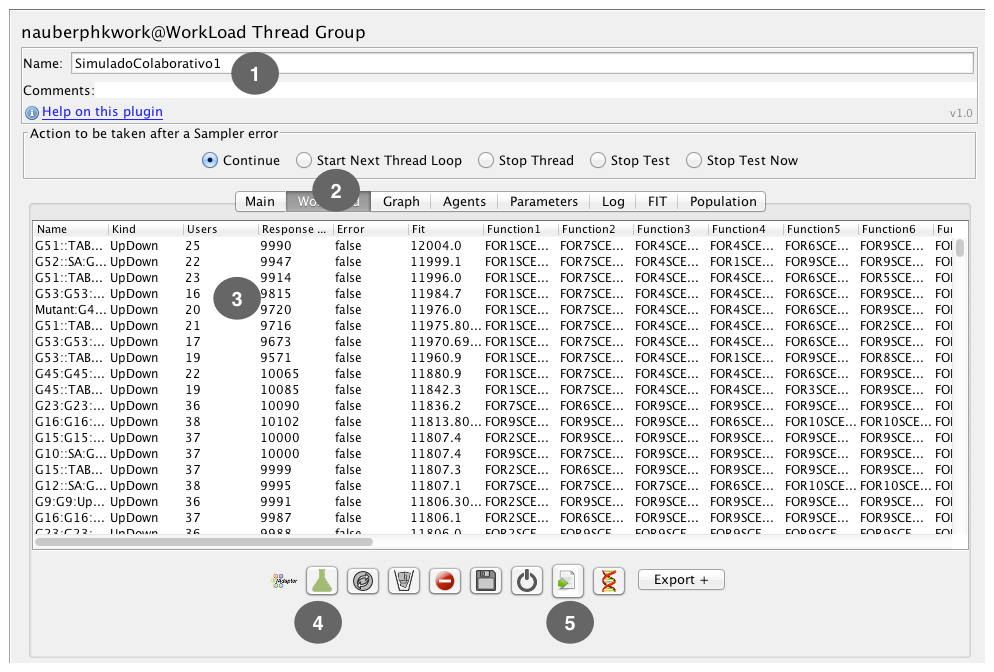
\includegraphics[width=0.5\textwidth]{./images/tela1iadapter.png}
\caption{WorkLoadThreadGroup component}
\label{fig:tela1iadapter}
\end{figure}

The WorkLoadSaver component is responsible for saving all data in the database. The operation of the component only requires its inclusion in the test script.

The WorkLoadController represents a scenario of test. The WorkLoadController represents a scenario of test. All actions necessary to test a application should be included in this component. All instance of the component need to login in the application under test and return the application to it's original state.
\section{Experiments}

This section presents two experiments. The first one has been applied in an emulated component and The second experiment has been applied in an installed Moodle application. The experiments used this fitnesse function:

\begin{equation}
\begin{aligned}
fit=0.9* 90percentiletime\\
+0.1*80percentiletime\\+
0.1*70percentiletime+\\
0.1*maxResponseTime+\\
0.2*numberOfUsers-penalty
\end{aligned}
\end{equation}

The fitnesse function used in the experiments intended to find individuals with the highest percentile of 90\%, followed by individuals with higher percentile time of 80\% and 70\%, maximum response time and number of users.

The first experiment has implemented 27 generations and the second experiment has performed 6 generations, with 300 executions by generation (100 times for each algorithm),  generating 300 new individuals. The experiments had used a initial population of 100 individuals. The Genetic Algorithm used the top 10 individuals from each generation to the crossover operation. The Tabu List has been configured with the size of 10 individuals and expire every 2 generations.  The mutation operation was applied to 10\% of the population on each generation. 

\subsection{First Experiment- Emulated Class Test}

The first experiment aimed to apply performance, load and stress testing in a simulated component. The purpose of using a simulated component is able to perform a greater number of generations in a shorter time available and eliminate variables such as the use of databases and application servers. The first experiment used a test class  named SimulateConcurrentAccess. These class have a static variable named \textit{x} and a set of methods that uses the variable in a synchronized context ( Listing \ref{classsimulated}).

\lstdefinestyle{outline}{
		language=Java,
         basicstyle=\scriptsize\ttfamily,
         numberstyle=\tiny,
         numbersep=5pt,
         tabsize=2,
         extendedchars=true,
         breaklines=true,
         keywordstyle=\color{black}\bf,
         frame=b,  % <<<<<<<<<<<<<<<<<<<<<<<<<<
         stringstyle=\color{green!40!black}\ttfamily,
         showspaces=false,
         showtabs=false,
         numbers=left,
         xleftmargin=17pt,
         framexleftmargin=17pt,
         framextopmargin=1pt, % <<<<<<<<<<<<<<<<<<<<<<
         showstringspaces=false,
         %backgroundcolor=\color[RGB]{200,200,200},
         belowcaptionskip=0pt
}

\begin{lstlisting}[style=outline,caption={SimulateConcurrentAcess class},float,label=classsimulated]
public class SimulateConcurrentAccess {
  @Test
  public void test() {		
    synchronized (StaticClass.class) {
			for (int i = 0; i <= 1000; i++) {
				StaticClass.x += i;
			}
			StaticClass.x = 0;
		}
	}
\end{lstlisting}


Fig.\ref{fig:exp1bestresults} presents the best results in 27 generations applied in the first experiment . The Figure shows the results obtained with the algorithms with and without collaboration. The $x$ axis  represents the generation number and the $y$ axis represents the best fitnesse value obtained until the current generation. The results of the experiment showed that the use of cooperation between the three algorithms resulted in find individuals with better fitnesse values.

\begin{figure}[h]
\centering
\caption{Best results obtained in 27 generations}
\includegraphics[width=0.5\textwidth]{./images/generationcomparative.png}
\label{fig:exp1bestresults}
\end{figure}
The table \ref{tab:averagefirst} presents the results obtained by the Hybrid Metaheuristc (HM), Genetic Algorithm (GA), Simulated Annealing (SA) and TABU Search (TS) from 27 generations in the first experiment. The values are the maximum value of the fitnesse obtained in each algorithm. 

\begin{table}[h]
\centering
\caption{Fitnesse function maximum value by algorithm}
\label{tab:averagefirst}
\begin{tabular}{|l|l|l|l|l|}
\hline
GEN & HM & TS  & GA    & SA    \\ \hline
1          & 11238 & 11238         & 11238 & 11238 \\ \hline
2          & 11804 & 11596         & 11801 & 10677 \\ \hline
3          & 11787 & 8932          & 8411  & 10869 \\ \hline
4          & 11723 & 9753          & 9611  & 10760 \\ \hline
5          & 8164  & 9780          & 10738 & 4794  \\ \hline
6          & 11802 & 9781          & 11086 & 6120  \\ \hline
7          & 9985  & 5782          & 11272 & 11798 \\ \hline
8          & 11803 & 11749         & 10084 & 11309 \\ \hline
9          & 11806 & 7284          & 11633 & 10766 \\ \hline
10         & 11807 & 9386          & 11717 & 4557  \\ \hline
11         & 11802 & 9653          & 11802 & 11151 \\ \hline
12         & 11807 & 10594         & 11793 & 9434  \\ \hline
13         & 11802 & 10848         & 10382 & 11805 \\ \hline
14         & 11801 & 11551         & 7219  & 10237 \\ \hline
15         & 11807 & 1701          & 7189  & 9338  \\ \hline
16         & 11813 & 6203          & 11758 & 5321  \\ \hline
17         & 11805 & 10720         & 10805 & 11748 \\ \hline
18         & 9600  & 6371          & 11698 & 7818  \\ \hline
19         & 11733 & 8160          & 11648 & 11509 \\ \hline
20         & 9589  & 9428          & 11805 & 4813  \\ \hline
21         & 11800 & 9463          & 11798 & 10801 \\ \hline
22         & 11805 & 11799         & 11804 & 6029  \\ \hline
23         & 11836 & 11655         & 11800 & 3579  \\ \hline
24         & 11805 & 11512         & 11803 & 5761  \\ \hline
25         & 11804 & 11573         & 11802 & 9680  \\ \hline
26         & 11800 & 11575         & 11403 & 9388  \\ \hline
27         & 11805 & 10691         & 11745 & 9465  \\ \hline
\end{tabular}
\end{table}

The signed-rank Wilcoxon non-parametrical procedure was used for comparing the results. The procedure showed that there was a significant improvement in the results with the collaborative approach.

\subsection{Second Experiment- Moodle Application Test}

The second experiment uses a Moodle application installed in a machine with 500 Gb of hard disk and 8 Gb of memory.The study used six application scenarios:

\begin{itemize}
\item PostDeleteMessage- This scenario post and delete messages in the moodle application.
\item MyHome- This scenario access the user's homepage of the application.
\item Login- This scenario are responsible by the user authentication of the application.
\item Notifications- This scenario enter in the notification page of each user.
\item Start Page- Initial start page of the application.
\item Badge- This scenario enter in the Badge page.
\end{itemize}

The maximum tolerated response time in test was 30 seconds.  Any  individuals that obtained a time longer than the stipulated maximum time suffered penalties.  The whole process of stress and performance tests, which took three days and about 1800 executions, was carried out without the need for monitoring of a test designer. The tool have  selected automatically the next scenarios to be run up to the limit of six generations previously established. 

The Table \ref{tab:secondexperiment} presents the maximum fitnesse value obtained by the Hybrid Metaheuristc (HM), Genetic Algorithm (GA), Simulated Annealing (SA) and TABU Search (TS) in each generation. 

\begin{table}[h]
\centering
\caption{Results obtained from the second experiment}
\label{tab:secondexperiment}
\begin{tabular}{|l|l|l|l|l|}
\hline
GEN & HM    & TS    & GA    & SA    \\
\hline
1          & 32242 & 32242 & 32242 & 32242 \\
\hline
2          & 34599 & 32443 & 26290 & 35635 \\
\hline
3          & 35800 & 34896 & 34584 & 34248 \\
\hline
4          & 35782 & 34912 & 32689 & 25753 \\
\hline
5          & 35611 & 31833 & 34631 & 8366  \\
\hline
6          & 35362 & 35041 & 33397 & 9706 \\
\hline
\end{tabular}
\end{table}


The small number of samples of the experiment is insufficient to give a statistical significance with Wilcoxon procedure. However, it is noted that in 4 of 6 generations, the collaborative approach presented the best values. The experiment succeeded in finding 29 individuals where the maximum time expected by the application was obtained.  The Table. \ref{tab:secondexperiment11} has a example of the six individuals with the highest fit values in the second experiment. The Table shows the fitnesse value (Fit),  the name of scenario (Scenario), the number of users (N.Users), the percentiles of 90\%,80\% and 70\% (90per, 80 per and 70per) in seconds.  

% Please add the following required packages to your document preamble:
% \usepackage{multirow}
\begin{table}[h]
\centering
\caption{Example of individuals obtained in the second experiment}
\label{tab:secondexperiment1}
\begin{tabular}{|l|l|l|l|l|l|l|}
\hline
Ind&Fit&Scenario&N.Users&90per&80per&70per\\ \hline
\multirow{2}{*}{1} & \multirow{2}{*}{35800} & MyHome        & 31              & \multirow{2}{*}{30} & \multirow{2}{*}{29} & \multirow{2}{*}{10} \\ \cline{3-4}
                   &                        & Badges        & 4               &                     &                     &                     \\ \hline
\multirow{3}{*}{2} & \multirow{3}{*}{35795} & MyHome        & 30              & \multirow{3}{*}{30} & \multirow{3}{*}{29} & \multirow{3}{*}{10} \\ \cline{3-4}
                   &                        & Notifications & 2               &                     &                     &                     \\ \cline{3-4}
                   &                        & Badges        & 2               &                     &                     &                     \\ \hline
\multirow{2}{*}{3} & \multirow{2}{*}{35782} & MyHome        & 32              & \multirow{2}{*}{30} & \multirow{2}{*}{29} & \multirow{2}{*}{10} \\ \cline{3-4}
                   &                        & Badges        & 3               &                     &                     &                     \\ \hline
\multirow{3}{*}{4} & \multirow{3}{*}{35773} & MyHome        & 22              & \multirow{3}{*}{30} & \multirow{3}{*}{29} & \multirow{3}{*}{10} \\ \cline{3-4}
                   &                        & Notifications & 6               &                     &                     &                     \\ \cline{3-4}
                   &                        & Badges        & 9               &                     &                     &                     \\ \hline
\multirow{2}{*}{5} & \multirow{2}{*}{35771} & MyHome        & 28              & \multirow{2}{*}{30} & \multirow{2}{*}{29} & \multirow{2}{*}{9}  \\ \cline{3-4}
                   &                        & Badges        & 6               &                     &                     &                     \\ \hline
\multirow{2}{*}{6} & \multirow{2}{*}{35683} & MyHome        & 27              & \multirow{2}{*}{30} & \multirow{2}{*}{29} & \multirow{2}{*}{8}  \\ \cline{3-4}
                   &                        & Badges        & 10              &                     &                     &                     \\ \hline
\end{tabular}
\end{table}

%\section{Contributions and Comparative Analysis}

The main contributions of the research are:

\begin{itemize}
\item The presentation of an approach that uses a committee of algorithms (GA, SA and TS);
\item The use of Tabu Search Algorithm ( TS ) to find scenarios that break the  service level defined by the application under test;
\end{itemize}

The secondary contributions of the research are:

\begin{itemize}
\item The provision of a JMeter plugin for conducting performance, load or stress  testing.
\item The extension of the survey conducted by  Afzal et al. in the Load, Performance and Stress testing context \cite{Afzal2009}
\item The automation of the  load, performance or stress test execution process.
\end{itemize}

The Figure \ref{fig:comparison} presents the comparison between this research and the others studies found in the systematic review. The IAdapter presents a solution that uses a committee of algorithms in a measurement approach using a functional tool (JMeter with IAdapter plugin).

\begin{figure}[h]
\centering
\includegraphics[width=0.5\textwidth]{./images/comparativo.png}
\caption{
Distribution of the researches over range of applied metaheuristics}
\label{fig:comparison}
\end{figure}
\section{Conclusion}

This paper presented a approach of use Hybrid Metaheuristc in load, performance and stress testing. Two experiments were performed to validate the solution. The first experiment has been applied in an emulated component and the second experiment has been applied in an installed Moodle application.  The collaborative approach has obtained better fit values in both experiments. 

The main contributions of the research are: The presentation of an approach that uses a hybrid metauristc to perform load, performance and stress tests;  The development of a JMeter plugin  to evolutionary tests and  the automation of the  load, performance or stress test execution process.

Among the future work of the research, we can highlight the use of new combinatorial optimization algorithms such as Very large-scale neighborhood search.

\bibliographystyle{plain}
\bibliography{sample.bib}

%\balancecolumns % GM June 2007
% That's all folks!
\end{document}